% ===========================================================================
% MAIN FILE — ML-MPC Wind Turbine Paper
% Amidou Maiga — Erciyes University
% Compile on Overleaf: pdflatex → bibtex → pdflatex → pdflatex
% ===========================================================================

\documentclass[12pt, a4paper]{article}

% ── Encoding & language ─────────────────────────────────────────────────────
\usepackage[utf8]{inputenc}
\usepackage[T1]{fontenc}
\usepackage[english]{babel}

% ── Mathematics ─────────────────────────────────────────────────────────────
\usepackage{amsmath, amssymb}

% ── Graphics & tables ───────────────────────────────────────────────────────
\usepackage{graphicx}
\usepackage{booktabs}
\usepackage{tabularx}
\usepackage{multirow}
\usepackage{multicol}
\usepackage{caption}
\usepackage{subcaption}
\usepackage[table]{xcolor}
\usepackage{float}
\usepackage{makecell}
\usepackage{tabularx}
\usepackage{booktabs}   %  \toprule, \midrule, \bottomrule
\usepackage{siunitx}     %  \SI\usepackage{tabularx}
\usepackage{booktabs}   %  \toprule, \midrule, \bottomrule
\usepackage{siunitx}     %  \SI


% ── Layout ──────────────────────────────────────────────────────────────────
\usepackage{geometry}
\geometry{a4paper, margin=2.5cm}
\usepackage{setspace}
\onehalfspacing
\usepackage{parskip}
\setlength{\parindent}{1cm}

% ── Lists ───────────────────────────────────────────────────────────────────
\usepackage{enumitem}

% ── Units ───────────────────────────────────────────────────────────────────
\usepackage{siunitx}
\sisetup{separate-uncertainty=true}

% ── Algorithm / pseudocode ───────────────────────────────────────────────────
\usepackage[ruled, vlined, linesnumbered]{algorithm2e}

% ── Hyperlinks ──────────────────────────────────────────────────────────────
\usepackage{hyperref}
\hypersetup{
    colorlinks = true,
    linkcolor  = blue,
    citecolor  = blue,
    urlcolor   = blue,
    pdftitle   = {Comparative Study of Machine Learning Surrogates for Nonlinear Model Predictive Control of Wind Turbine Rotor Speed in Above-Rated Operation},
    pdfauthor  = {Amidou Maiga},
}

% ── Bibliography ────────────────────────────────────────────────────────────
\usepackage{natbib}
\bibliographystyle{unsrtnat}

% ── Table font size ─────────────────────────────────────────────────────────
\usepackage{etoolbox}
\AtBeginEnvironment{table}{\small}

% ── Custom commands (shared across all sections) ─────────────────────────────
\newcommand{\omegar}{\omega_r}
\newcommand{\omegarated}{\omega_{\text{rated}}}
\newcommand{\Tg}{T_g}
\newcommand{\Ta}{T_a}
\newcommand{\Kopt}{K_{\text{opt}}}
\newcommand{\Cp}{C_p}
\newcommand{\betacmd}{\beta_{\text{cmd}}}
\newcommand{\RMSE}{\text{RMSE}}
%\newcommand{\deg}{^{\circ}}

% ===========================================================================
% TITLE PAGE
% ===========================================================================
\title{
    \Large\textbf{Comparative Study of Machine Learning Surrogates for
    Nonlinear Model Predictive Control of Wind Turbine Rotor Speed
    in Above-Rated Operation}
}

\author{
	\textbf{Amidou Maiga},
	\textbf{Mustafa Serdar GENÇ},
	\textbf{Gamze GENÇ},\\
	\textbf{Ahmet AKSÖZ},
	\textbf{Dongran Song},   
}

%\author{
%	\textbf{Amidou Maiga}\\[0.4em]
%	\small Department of Energy Systems Engineering\\
%	\textbf{Mustafa Serdar GENÇ}\\[0.4em]
%	\small Department of Energy Systems Engineering\\
%	\small Erciyes University, Kayseri, Turkey\\[0.5em]
%	\textbf{Gamze GENÇ}\\[0.4em]
%	\small Department of Energy Systems Engineering\\
%	\small Erciyes University, Kayseri, Turkey\\   [0.5em]
%	\textbf{Ahmet AKSÖZ}\\[0.4em]
%	\small Department of Electrical-Electronic Engineering\\
%	\small Kayseri University, Kayseri, Turkey\\ [0.5em]
%	\textbf{Dongran Song}\\[0.4em]
%	\small Department of Electrical-Electronic Engineering\\
%	\small Central South University, Changsha, China\\   
%}

\date{}

% ===========================================================================
\begin{document}

\maketitle
\thispagestyle{empty}

% ── Abstract ────────────────────────────────────────────────────────────────
% ===========================================================================
% ABSTRACT
% ===========================================================================

\begin{abstract}
Wind turbine speed regulation in above-rated operation requires fast,
constraint-aware control; nonlinear Model Predictive Control (MPC) is
well suited to this, but its internal plant model is expensive to
evaluate at every step, motivating cheaper learned surrogates. We
compare six surrogate architectures --- LLNFM, LSTM, GP, PINN, TCN, and
SW-MLP --- as internal predictors in a nonlinear MPC for the NREL 5-MW
turbine. One-step prediction accuracy and closed-loop tracking prove
only loosely coupled. What initially appeared as a hard operational
incompatibility between LSTM/TCN/SW-MLP/PINN-v2/GP-v2 and SQP-based
\texttt{nlmpc} was traced, through a five-stage diagnostic, to
repeated \texttt{predict()} calls inside the solver --- not
architecture, model size, or MATLAB version. Independently,
\texttt{predict()}'s single-precision output was found to zero out
\texttt{fmincon}'s default finite-difference gradient estimate for
two of these architectures, corrupting solver feasibility regardless
of any real-time deadline. A verified manual forward
pass, computed in double precision, restored closed-loop viability for
all six surrogates. All
results hold under two explicit conditions: a bounded
thirty-iteration SQP solver budget, and a single software toolchain
(MATLAB Deep Learning Toolbox, tested on releases R2024a and R2026a) ---
no cross-toolchain replication was performed. On an Intel Core
i5-12450H (12th Gen, 16\,GB RAM) under R2024a, the headline result is a
$491\times$ mean per-step speedup for LSTM, the largest of the six
architectures tested (full range: $5.5\times$--$491\times$). We further identify a
Region~II/III torque-switching correction as a precondition for stable
closed-loop simulation, and, applying the same diagnostic rigor to our
own results, find that a previously reported "zero pitch activity"
result for a Mat\'ern-kernel GP uncertainty-penalized MPC cost is in
fact a solver-infeasibility artifact (a frozen actuator command, not
genuine regulation) rather than a controller achievement --- a finding
we report as a caution against under-instrumented closed-loop
comparisons, consistent with the diagnostic ethos of this paper.
These results reframe an apparent architectural limitation as a
diagnosable, remediable implementation cost, with practical guidance
for deploying ML surrogates in real-time MPC.

\textbf{Keywords:} Model Predictive Control, Wind Turbine Control,
Machine Learning Surrogates, Gaussian Process, Real-Time Feasibility
\end{abstract}

\newpage

% ── Table of contents ───────────────────────────────────────────────────────
\tableofcontents
\newpage

% ── Sections ────────────────────────────────────────────────────────────────
% ===========================================================================
% SECTION 1 — INTRODUCTION
% Target: 800-1000 words
% ===========================================================================

\section{Introduction}
\label{sec:introduction}

Wind energy is one of the fastest-growing renewable energy sources, and
the continued growth of installed capacity places increasing demands on
turbine control systems \citep{pao2009}. Above the rated wind speed
(Region~III), a variable-speed, variable-pitch wind turbine must regulate
rotor speed to its rated value by actuating blade pitch, while the
generator torque is held at (or switched into) its rated value
\citep{bianchi2006}. This regulation problem is nonlinear, subject to
actuator rate and range constraints, and driven by a highly stochastic
disturbance (turbulent wind); Model Predictive Control (MPC) is
well-suited to it precisely because it handles input and state
constraints explicitly and can anticipate disturbance effects over a
prediction horizon \citep{rawlings2017}, in contrast to classical
gain-scheduled PI pitch
controllers \citep{bianchi2006,pao2009,laks2009}. The practical obstacle to
nonlinear MPC (NMPC) for this problem is computational: at every control
step, the solver must repeatedly evaluate the internal plant model — and,
for gradient-based solvers, its Jacobian — which is expensive when that
model is the full nonlinear aerodynamic and structural dynamics of the
turbine \citep{schlipf2013,evans2022}.

\subsection{ML-MPC: State of the Art}
\label{subsec:soa}

A natural response to this computational bottleneck is to replace the
physical plant model inside the MPC prediction step with a learned
surrogate that is cheaper to evaluate. \citet{klein2024,klein2025} recently
demonstrated this approach for wind turbine load-relevant control using a
Local Linear Neuro-Fuzzy Model (LLNFM) surrogate inside an adaptive MPC
framework, validated on a full-scale turbine — the direct reference and
starting point for the two-state modeling and LLNFM implementation adopted
in this work (Section~\ref{sec:system_modeling}). Beyond neuro-fuzzy
surrogates, Gaussian Process (GP) regression has an established track
record as an MPC-internal model precisely because it returns a calibrated
predictive uncertainty alongside its point prediction, enabling cautious
or uncertainty-aware control formulations \citep{kocijan2004,hewing2020} —
a property we exploit directly in the GP-based cost of
Section~\ref{subsec:gp_uncertainty_cost}. Within wind energy specifically,
\citet{liu_wind_2018} use a Mat\'ern-kernel GP to predict short-term wind
speed for preview-based load mitigation, but --- unlike the present
work --- as an external disturbance forecast feeding the controller
rather than as the MPC's internal dynamics model. Data-driven
reinforcement learning has separately been applied to wind turbine
torque/pitch control \citep{xie_data-driven_2023}, offering a
model-free alternative to the surrogate-based MPC approach studied
here; we return to this comparison in
Section~\ref{sec:discussion}. Physics-Informed Neural Networks
(PINNs), which embed a governing differential equation as a soft
constraint on the training loss, have become a general framework for
combining data-driven flexibility with physical consistency
\citep{raissi2019,karniadakis2021}, and Temporal Convolutional Networks
(TCNs) have been shown to be a competitive, often superior alternative to
recurrent architectures for generic sequence modeling tasks
\citep{bai2018}. Each of these four paradigms — neuro-fuzzy, GP, PINN,
and convolutional/recurrent sequence models — has therefore been
independently validated as a plausible MPC surrogate architecture in some
application domain. Beyond ML surrogates specifically, the broader
engineering practice of MPC continues to evolve rapidly
\citep{schwenzer2021}, and linear-quadratic-optimal alternatives to
nonlinear MPC for wind turbine power tracking, without a learned
internal model, have also recently been proposed and validated in
OpenFAST \citep{grapentin2022,grapentin2024} --- a useful point of
comparison for the computational-cost trade-offs discussed in
Section~\ref{sec:mpc_framework}, though outside this paper's
ML-surrogate scope.

What is missing, to our knowledge, is a systematic comparison of these
paradigms \emph{within a single closed-loop MPC framework, on the same
plant, under the same solver}, paired with an explicit operational
feasibility analysis of running each surrogate inside a real-time SQP
solve rather than only an open-loop accuracy comparison. Prior work
typically evaluates one surrogate family in isolation
\citep{klein2024,kocijan2004,hewing2020}; the interaction between
surrogate architecture and the specific numerical behavior of a
gradient-based NMPC solver — which, as we show in
Section~\ref{subsec:operational_feasibility}, can render an
otherwise-accurate surrogate practically unusable — is, to our knowledge,
not addressed in the existing wind turbine ML-MPC literature.

\subsection{Contributions}
\label{subsec:contributions}

This paper makes four contributions:

\begin{enumerate}
\item A systematic comparison of six ML surrogate architectures (LLNFM,
LSTM, GP, PINN, TCN, SW-MLP) as internal state predictors for nonlinear
MPC of wind turbine rotor speed, evaluated both open-loop (one-step
prediction accuracy) and closed-loop (tracking performance under
turbulent wind), across two model generations (V1, V2).
\item An operational feasibility analysis documenting a hard
incompatibility between \texttt{dlarray}-based deep-learning surrogates
and SQP-based \texttt{nlmpc} in MATLAB R2024a, driven by non-deterministic
JIT recompilation rather than a soft accuracy-cost trade-off, with
per-call and per-solve timing evidence.
\item A Region~II/III generator torque switching correction for the
two-state plant model, calibrated at the turbine's actual rated operating
point rather than its theoretical aerodynamic optimum, without which
long-horizon closed-loop simulation enters an irrecoverable operating
trap — a modeling detail we show is not a minor implementation nicety but
a precondition for valid training data and closed-loop evaluation.
\item A Gaussian-Process-based uncertainty-penalized MPC cost, made
statistically meaningful through Matérn~5/2 kernel selection and Bayesian
hyperparameter optimization, extending the cautious-MPC literature
\citep{hewing2020,kocijan2004} to Region~III wind turbine speed
regulation.
\end{enumerate}

\subsection{Paper Organization}
\label{subsec:organization}

Section~\ref{sec:system_modeling} presents the plant, torque-switching,
and wind models. Section~\ref{sec:dataset_generation} describes the
training data generation protocol. Section~\ref{sec:ml_surrogates}
details all six surrogate architectures and their open-loop accuracy.
Section~\ref{sec:mpc_framework} presents the NMPC formulation, surrogate
integration, and operational feasibility analysis. Section~\ref{sec:closed_loop_results}
reports closed-loop V1 and V2 results, their comparison, and a Monte Carlo
robustness analysis. Section~\ref{sec:discussion} discusses the main
findings, limitations, and directions for future work, and
Section~\ref{sec:conclusion} concludes.

\newpage

% ===========================================================================
% SECTION 2 — SYSTEM MODELING
% Target: 600-800 words
% ===========================================================================

\section{System Modeling}
\label{sec:system_modeling}

\subsection{NREL 5-MW Reference Turbine}
\label{subsec:nrel5mw}

This study uses the NREL offshore 5-MW reference wind turbine
\citep{jonkman2009} as the physical plant. This model is widely adopted as a
benchmark in the wind energy control literature, which allows direct
comparison with previously published MPC and ML-surrogate studies. The
turbine has a rotor radius $R = \SI{63}{m}$, a combined drivetrain inertia
$J = 3.876 \times 10^{7}~\text{kg}\cdot\text{m}^2$ (referred to the
low-speed shaft, LSS), a $97{:}1$ gearbox ratio, a rated rotor speed
$\omegarated = \SI{12.1}{rpm}$, and a rated generator torque (high-speed
shaft, HSS) $T_{g,\text{rated}} = P_{\text{rated}} / (\omegarated
N_{\text{gear}}) = \SI{40680}{N.m}$. The rated tip-speed ratio is
$\lambda_{\text{rated}} = 7.00$. Full turbine parameters are reported in
Table~\ref{tab:turbine_params}.

\begin{table}[H]
\centering
\caption{NREL 5-MW reference turbine parameters used in this study
(source: \citet{jonkman2009}, with the drivetrain damping and torque
switching calibration choices documented in Section~\ref{subsec:torque_switching}).}
\label{tab:turbine_params}
\begin{tabular}{lcc}
\toprule
Parameter & Symbol & Value \\
\midrule
Rotor radius              & $R$                 & \SI{63}{m} \\
Number of blades          & $B$                 & 3 \\
Air density                & $\rho$              & \SI{1.225}{kg/m^3} \\
Drivetrain inertia (LSS)   & $J$                 & $3.876\times10^{7}$ kg$\cdot$m$^2$ \\
Drivetrain damping         & $B_r$               & \SI{6215.5}{N.m.s/rad} \\
Gear ratio                 & $N_{\text{gear}}$   & 97 \\
Pitch actuator time constant & $\tau_\beta$      & \SI{0.1}{s} \\
Pitch bounds                & $\beta$             & $[0,\ 25]\deg$ \\
Maximum pitch rate          & $\dot\beta_{\max}$  & \SI{8.0}{deg/s} \\
Rated rotor speed          & $\omegarated$       & \SI{12.1}{rpm} \\
Physical min.\ rotor speed & $\omega_{\min}$     & \SI{4.77}{rpm} \\
Overspeed limit (+10\%)    & $\omega_{\max}$     & \SI{13.31}{rpm} \\
Rated tip-speed ratio       & $\lambda_{\text{rated}}$ & 7.00 \\
Rated power                & $P_{\text{rated}}$  & \SI{5}{MW} \\
Rated wind speed           & $V_{\text{rated}}$  & \SI{11.4}{m/s} \\
Cut-in wind speed          & $V_{\text{in}}$     & \SI{3.0}{m/s} \\
Cut-out wind speed         & $V_{\text{out}}$    & \SI{25.0}{m/s} \\
Rated generator torque (HSS) & $T_{g,\text{rated}}$ & \SI{40680}{N.m} \\
Region II gain (LSS)        & $\Kopt$             & $2.5106\times10^{6}$~N.m.s$^2$ \\
\bottomrule
\end{tabular}
\end{table}

\subsection{Two-State Model}
\label{subsec:two_state_model}

Following the modeling approach of \citet{klein2024}, the turbine is
represented by a reduced two-state nonlinear model with state vector
$x = [\omegar, \beta]^\top$, control input $u = \betacmd$ (pitch angle
demand), and measured disturbance $V$ (rotor-effective wind speed). The
rotor dynamics are governed by the aerodynamic torque balance

\begin{equation}
J\,\dot{\omegar} = \Ta(\omegar, \beta, V) - \Tg^{\text{LSS}}(\omegar) - B_r\,\omegar,
\label{eq:rotor_ode}
\end{equation}

where $\Tg^{\text{LSS}}$ is the generator reaction torque referred to the
low-speed shaft (Section~\ref{subsec:torque_switching}), $B_r =
\SI{6215.5}{N.m.s/rad}$ is a linear drivetrain damping coefficient
(Table~\ref{tab:turbine_params}), and the
aerodynamic torque is
$\Ta = \tfrac{1}{2}\rho \pi R^2 V^3 \Cp(\lambda,\beta) / \omegar$, with tip-speed
ratio $\lambda = \omegar R / V$ and power coefficient surface
$\Cp(\lambda,\beta)$ evaluated with the Jonkman polynomial. The pitch
actuator is modeled as a first-order lag,

\begin{equation}
\tau_\beta\,\dot{\beta} = \betacmd - \beta,
\label{eq:pitch_actuator}
\end{equation}

with $\tau_\beta = \SI{0.1}{s}$. Equations~\eqref{eq:rotor_ode}--\eqref{eq:pitch_actuator}
are integrated with explicit Euler discretization at $\Delta t = \SI{0.1}{s}$,
matching the control sampling time $T_s$ used by the nonlinear MPC in
Section~\ref{sec:mpc_framework}. The $\Cp(\lambda,\beta)$ surface is
evaluated strictly within its calibration domain $\beta \in [0\deg, 25\deg]$;
Stage~0 validation confirmed a maximum power coefficient
$\Cp^{\max} = 0.480$ at $\lambda^{*} = 8.11$, $\beta^{*} = 0\deg$, safely
below the Betz limit ($C_{p,\text{Betz}} = 0.5926$), correcting an earlier
non-physical evaluation of the polynomial outside its calibrated range that
had produced $\Cp^{\max} = 0.706 > C_{p,\text{Betz}}$.

\subsection{Region II/III Generator Torque Switching}
\label{subsec:torque_switching}

A methodological contribution of this work concerns the generator torque
model $\Tg^{\text{LSS}}(\omegar)$ in Eq.~\eqref{eq:rotor_ode}. An initial
implementation assumed a constant rated torque
$\Tg^{\text{LSS}} = N_{\text{gear}}\,T_{g,\text{rated}}$ at all rotor
speeds. Under this assumption, long-horizon closed-loop simulation revealed
an irrecoverable operating trap: for $\omegar$ below the rated speed, the
aerodynamic torque $\Ta$ available at low wind speed can fall below the
constant demanded generator reaction torque, driving $\dot{\omegar} < 0$
with no control authority left to arrest the deceleration (the pitch angle
is already saturated at its lower bound $\beta = 0\deg$), so the rotor
stalls toward zero speed.

This was corrected by replacing the constant-torque assumption with the
standard Region~II/III generator torque switching law, expressed
consistently in low-speed-shaft (LSS) torque on both sides,

\begin{equation}
\Tg^{\text{LSS}}(\omegar) =
\begin{cases}
\Kopt\,\omegar^{2}, & \omegar < \omegarated \quad \text{(Region II)} \\[4pt]
N_{\text{gear}}\,T_{g,\text{rated}}, & \omegar \geq \omegarated \quad \text{(Region III)}
\end{cases}
\label{eq:torque_switching}
\end{equation}

where $\Kopt = \tfrac{1}{2}\rho A_{\text{rotor}} \Cp(\lambda_{\text{rated}})
R^3 / \lambda_{\text{rated}}^3 = 2.5106\times10^{6}~\text{N.m.s}^2$ is
calibrated at the actual Jonkman operating point
$\lambda_{\text{rated}} = R\,\omegarated / V_{\text{rated}} = 7.00$, rather
than the theoretical aerodynamic optimum $\lambda^{*} = 8.11$ identified in
Section~\ref{subsec:two_state_model}. This choice follows standard practice
\citep[e.g.][]{jonkman2009}: Jonkman's rated operating point already
accounts for drivetrain and electrical losses, so it sits slightly off the
pure-aerodynamic $\Cp$ peak; calibrating $\Kopt$ there prioritizes torque
continuity at the switching boundary over exact aerodynamic optimality
(calibrating instead at $\lambda^{*}=8.11$ would produce a $30\%$
discontinuity, versus $2.26\%$ at $\lambda_{\text{rated}}=7.00$). The
resulting continuity ratio is
$\Kopt \omegarated^{2} / (N_{\text{gear}} T_{g,\text{rated}}) = 1.0226$,
i.e.\ a $2.26\%$ torque discontinuity at $\omegar = \omegarated$
(a single-point deficit of \SI{89108}{N.m} on the low-speed shaft,
$K_{\text{opt}}\omegarated^2 - N_{\text{gear}}T_{g,\text{rated}} =
\SI{4035098}{N.m} - \SI{3945990}{N.m}$), which is documented and accepted as
negligible: the explicit-Euler integration together with continuous
turbulent-wind excursions means the simulated system never dwells exactly
at $\omegar = \omegarated$ to machine precision. Feasibility of
Eq.~\eqref{eq:torque_switching} was validated by confirming
$\Ta(\omegar,\beta,V) - \Tg^{\text{LSS}}(\omegar) > 0$ for all
$\omegar \in [\omega_{\min}, \omegarated]$ and all $V$ in the operating
envelope, eliminating the trap. Fig.~\ref{fig:torque_switching} illustrates
$\Ta$ and $\Tg^{\text{LSS}}(\omegar)$ before and after the correction. This
correction also constrains the admissible rotor-speed range used for
surrogate-based MPC bounds in Stage~3
(Section~\ref{sec:mpc_framework}): the training domain identified in
Stage~1 (Section~\ref{sec:dataset_generation}) is $[8.02,13.31]$~rpm,
yielding surrogate MPC bounds of $[8.52,12.81]$~rpm with a
$\SI{0.5}{rpm}$ safety margin on each side, distinct from the wider
$[11.5,13.31]$~rpm defense-in-depth bound retained for the physics-based
Baseline controller.

\begin{figure}[H]
\centering
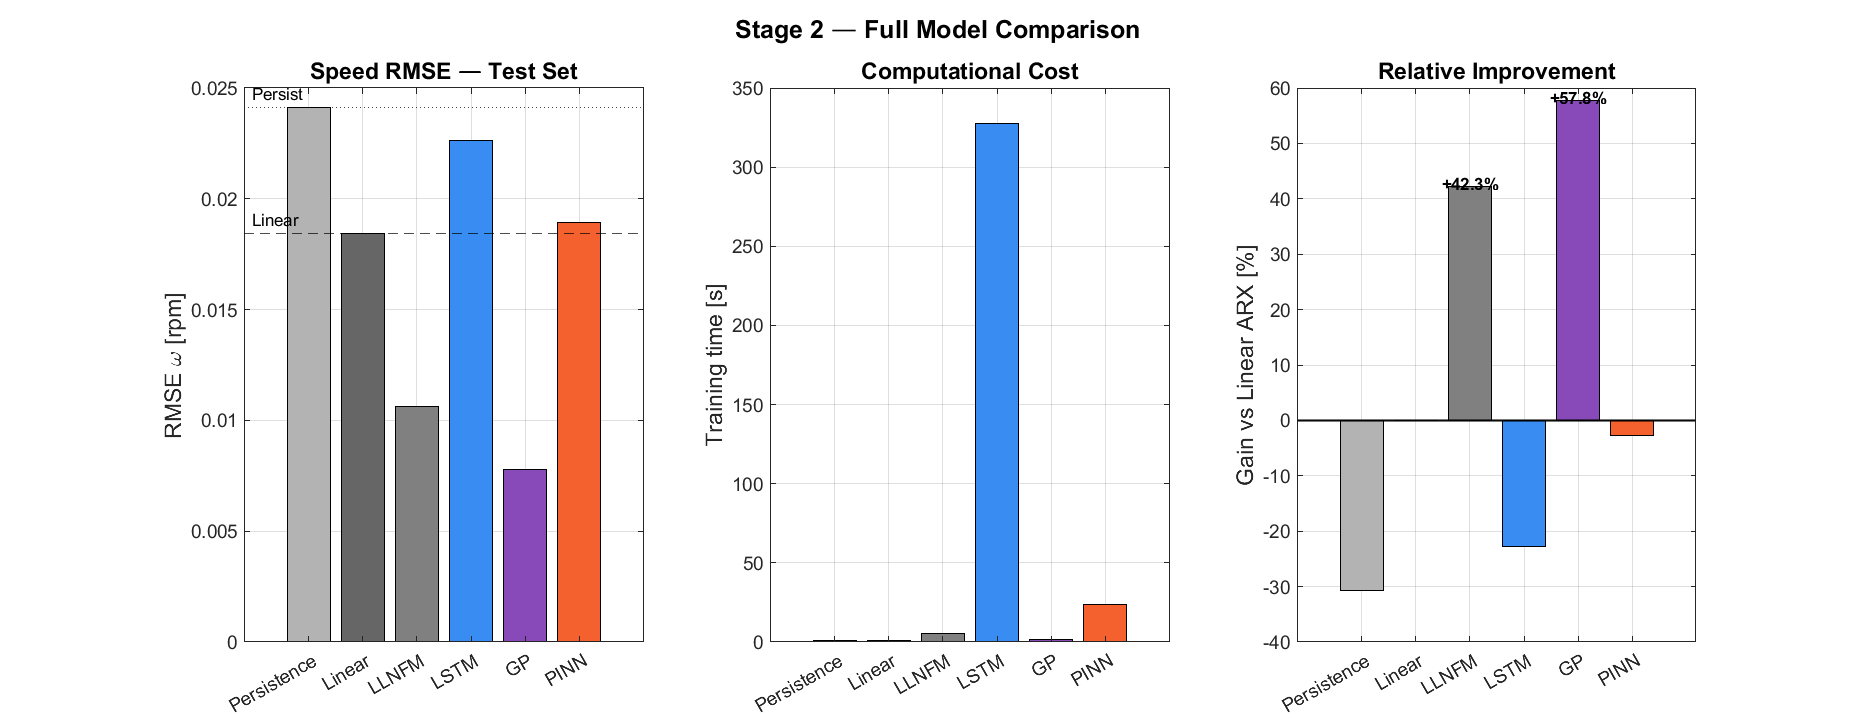
\includegraphics[width=0.8\textwidth]{figures/Fig3_S2_ModelSummary.png}
\caption{Region II/III generator torque switching: aerodynamic torque
$\Ta$ and generator torque $\Tg(\omegar)$ before (constant torque) and
after (Eq.~\eqref{eq:torque_switching}) correction.}
\label{fig:torque_switching}
\end{figure}

\subsection{Wind Model}
\label{subsec:wind_model}

Turbulent wind input is generated from the Kaimal spectrum defined in
IEC~61400-1 \citep{iec61400} with turbulence intensity $I = 0.16$,
longitudinal turbulence length scale $L_1 = \SI{340.2}{m}$. We note that
$I=0.16$ corresponds to IEC Turbulence Category~A (the more severe of
the two standard categories at this hub height) rather than
Category~B ($I=0.14$) as an earlier draft of this work mislabeled it;
the simulated turbulence is therefore somewhat more severe than a
Category-B label would imply, not less. Time series are
synthesized via inverse FFT of the discretized Kaimal power spectral
density, with the amplitude spectrum deterministically rescaled before
phase randomization so that the achieved standard deviation
$\sigma_{\text{actual}}$ matches the target
$\sigma_{\text{target}} = I \cdot V_{\text{mean}}$ \emph{by construction}
 this rescaling step is a normalization procedure, not an
independent validation of the synthesized turbulence, and should not
be read as evidence that the resulting time series matches the target
Kaimal spectrum in any property other than its overall standard
deviation; validating the achieved power spectral density shape
against the analytical Kaimal spectrum independently is noted as
future work. The
synthesized wind signal is subsequently passed through a second-order
Butterworth low-pass filter with cutoff frequency $f_c = \SI{0.3}{Hz}$,
consistent with the rotor-effective wind filtering approach of
\citet{klein2024}, before being applied as the disturbance input $V$ to
Eq.~\eqref{eq:rotor_ode}.

\newpage

% ===========================================================================
% SECTION 3 — DATASET GENERATION
% Target: 400-500 words
% ===========================================================================

\section{Dataset Generation}
\label{sec:dataset_generation}

\subsection{Simulation Protocol}
\label{subsec:simulation_protocol}

Training data for the machine learning surrogates is generated by
open-loop simulation of the two-state plant model
(Section~\ref{subsec:two_state_model}) under Region~II/III torque
switching (Section~\ref{subsec:torque_switching}). A total of $80$
trajectories of $300$ time steps each are simulated at $\Delta t =
\SI{0.1}{s}$, giving $80 \times 300 = 24{,}000$ samples. Each trajectory
uses a distinct mean wind speed $V_{\text{mean}}$, superimposed with a
turbulent Kaimal component (Section~\ref{subsec:wind_model}), and a
distinct pitch operating point $\beta_{\text{op}}$; across the 80
trajectories $V_{\text{mean}}$ spans the above-rated envelope up to the
cut-out region (e.g.\ $V_{\text{mean}} = \SI{14.3}{m/s}$ with
$\beta_{\text{op}} = 5.8\deg$ up to $V_{\text{mean}} = \SI{23.9}{m/s}$ with
$\beta_{\text{op}} = 25.0\deg$). The pitch input is excited with a
pseudo-random binary sequence (PRBS), $f_{\text{switch}} = \SI{0.5}{Hz}$,
step amplitude $\delta \in [1,3]\deg$, so that the surrogate training set
captures the local input-output sensitivity needed for one-step-ahead
prediction. Rotor speed initialization is deliberately widened down into
Region~II ($\omegar$ as low as $\approx\SI{8}{rpm}$, consistent with the
torque-switching-constrained range identified in
Section~\ref{subsec:torque_switching}) so that the resulting surrogates
generalize across the Region~II/III boundary rather than only in
above-rated operation.

\subsection{Dataset Structure}
\label{subsec:dataset_structure}

Each sample consists of a feature vector
$X = [\omegar,\ \beta,\ V,\ u_{\text{cmd}}]$ and a one-step-ahead target
$Y = [\omegar^{+},\ \beta^{+}]$, where $u_{\text{cmd}} = \betacmd$ is the
pitch demand applied at the current step and the superscript $+$ denotes
the state at $t+\Delta t$. The $24{,}000$ samples are split at the
\emph{trajectory} level, not the sample level, into $56$ training, $12$
validation, and $12$ test trajectories ($70\%/15\%/15\%$, random seed
$42$), giving $16{,}800$ training, $3{,}600$ validation, and $3{,}600$ test
samples. Splitting by trajectory rather than by individual sample preserves
temporal continuity within each subset and prevents information leakage
across adjacent time steps of the same trajectory, which is essential for a
fair evaluation of the sequence-based surrogates (LSTM, TCN,
Section~\ref{sec:ml_surrogates}) that would otherwise see near-duplicate
windows straddling the train/test boundary. Feature and target
normalization ($z$-score) is computed exclusively on the training split and
applied identically to validation and test data, avoiding any leakage of
validation/test statistics into the training pipeline.

\subsection{Feature Statistics}
\label{subsec:feature_statistics}

Table~\ref{tab:feature_stats} summarizes the operating envelope covered by
the generated dataset. The rotor speed ranges from $\SI{10.28}{rpm}$ to
$\SI{13.31}{rpm}$ (the upper bound coinciding with the plant's maximum
admissible speed, Section~\ref{subsec:nrel5mw}), the pitch angle spans its
full physical domain $[0,25]\deg$, and the wind speed ranges from
$\SI{7.85}{m/s}$ to the cut-out limit of $\SI{25.0}{m/s}$. The maximum
sampled power coefficient is $\Cp^{\max} = 0.480$, consistent with the
Stage~0 Betz-limit validation (Section~\ref{subsec:two_state_model}) and
confirming that no sample in the dataset violates aerodynamic feasibility.
A full dataset validation pass additionally confirmed the absence of
NaN/Inf values, physically consistent one-step increments
($\Delta\omegar$: mean $\SI{0.0030}{rpm}$, std $\SI{0.0217}{rpm}$, max
$\SI{0.1273}{rpm}$ per step; $\Delta\beta$: mean $-0.0006\deg$, std
$0.3250\deg$, max $0.8000\deg$ per step, consistent with the pitch rate
limit $\dot\beta_{\max}$), and correctly normalized training features
(zero mean, unit variance).

\begin{table}[H]
	\centering
	\caption{Dataset feature statistics (24{,}000 samples, 80 trajectories).}
	\label{tab:feature_stats}
	\begin{tabular}{lccc}
		\toprule
		Feature & Min & Max & Unit \\
		\midrule
		$\omegar$ & 10.28 & 13.31 & rpm \\
		$\beta$   & 0.00  & 25.00 & deg \\
		$V$       & 7.85  & 25.00 & m/s \\
		$u_{\text{cmd}}$ & 0.00 & 25.00 & deg \\
		$\Cp$ (sample max) & \multicolumn{2}{c}{0.480 (Betz = 0.5926)} & -- \\
		\bottomrule
	\end{tabular}
\end{table}

\begin{figure}[H]
	\centering
	 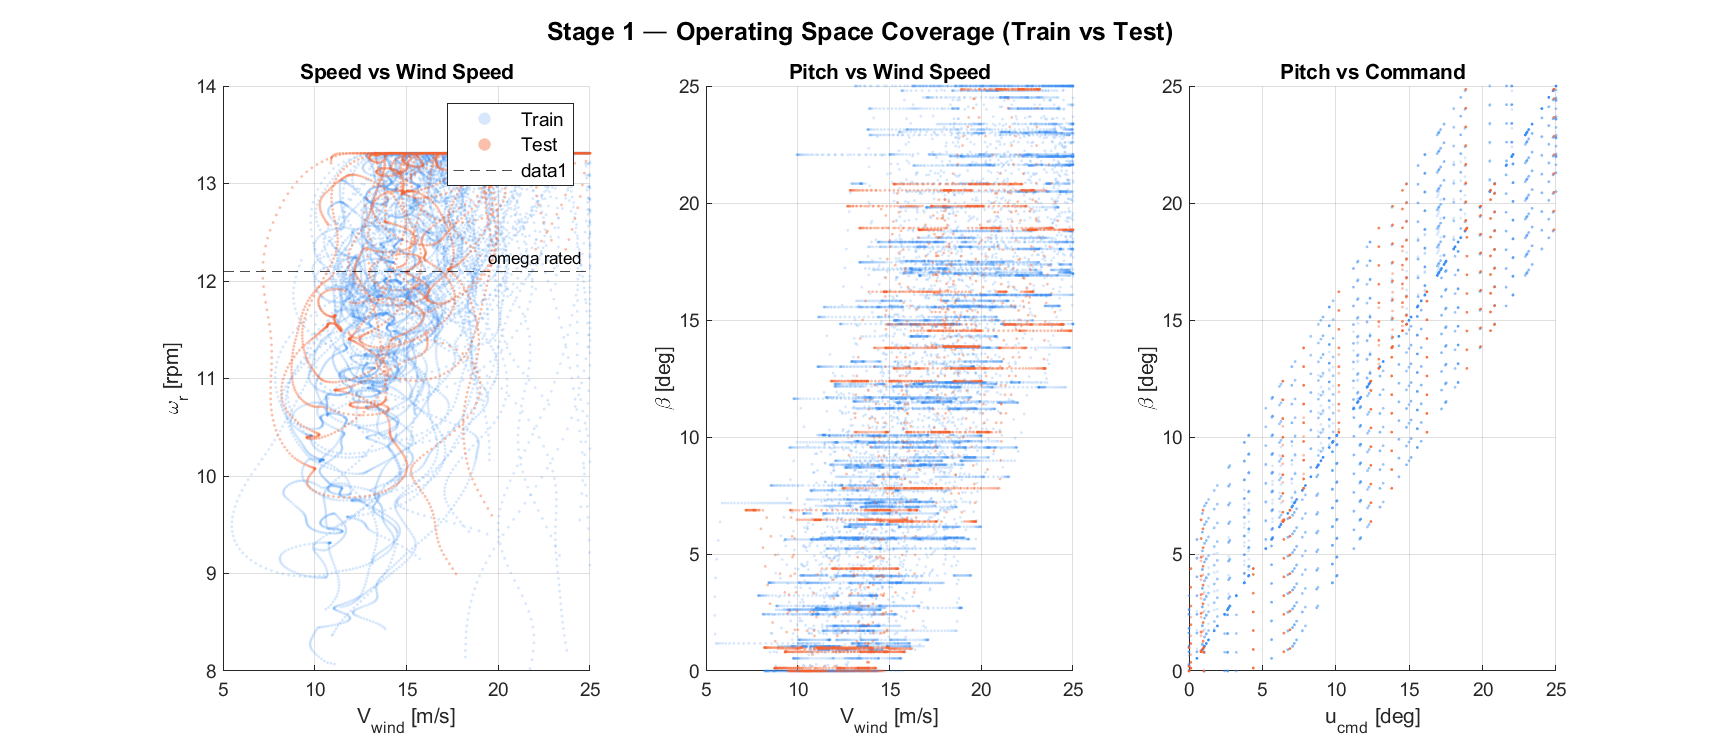
\includegraphics[width=1\textwidth]{figures/Fig1_S1_Coverage.png}
	\caption{Operating-space coverage of the generated dataset: rotor speed
		$\omegar$ versus wind speed $V$, training set (56 trajectories) versus
		test set (12 trajectories).}
	\label{fig:dataset_coverage}
\end{figure}
\newpage

% ===========================================================================
% SECTION 4 — MACHINE LEARNING SURROGATE MODELS
% Target: 1500-2000 words
% ===========================================================================

\section{Machine Learning Surrogate Models}
\label{sec:ml_surrogates}

All surrogates are trained on the Stage~1 dataset
(Section~\ref{sec:dataset_generation}) to predict the one-step-ahead state
$[\omegar^{+},\beta^{+}]$ from $X=[\omegar,\beta,V,u_{\text{cmd}}]$, using the
shared global normalization computed on the training split. Two naive
baselines are reported for reference: \emph{Persistence}
($\hat{x}^{+}=x$) and a \emph{Linear ARX} model fitted by ordinary least
squares. All six surrogate architectures below are trained and evaluated
under the same protocol.

\subsection{V1 Models}
\label{subsec:v1_models}

\subsubsection{Local Linear Neuro-Fuzzy Model (LLNFM / ANFIS)}
\label{subsubsec:llnfm}

The LLNFM surrogate is implemented as two independent Sugeno-type
ANFIS \citep{jang_anfis_1993} networks (one per output channel), each
with a grid-partitioned rule base
of $2$ generalized bell membership functions (\texttt{gbellmf}) per input,
giving $2^4=16$ fuzzy rules, $55$ network nodes, and $104$ total parameters
($80$ linear consequent parameters, $24$ nonlinear premise parameters).
Training uses MATLAB's \texttt{anfis()} function on a $3{,}000$-point
subsample of the training set for $80$ epochs. We note that the
\texttt{tunefis()} API (the object-oriented ANFIS training interface
introduced in recent MATLAB releases) proved incompatible in R2024a and
could not be used; the legacy matrix-based \texttt{anfis()} syntax was
confirmed to work correctly and was used throughout this study. The omega
sub-network converges quickly (error goal reached at epoch~2), while the
beta sub-network trains for the full $80$ epochs without reaching the error
goal, oscillating around a training RMSE of $\approx 0.013$--$0.017$ in
normalized units. Despite this, LLNFM achieves the best test-set accuracy
among all V1 surrogates: $\RMSE_{\omega} = \SI{0.0069}{rpm}$,
$\RMSE_{\beta} = 0.0936\deg$, in $\SI{5.8}{s}$ of training time.

\subsubsection{Gaussian Process (V1)}
\label{subsubsec:gp_v1}

The V1 Gaussian Process surrogate uses a Squared-Exponential (SE) kernel
with default (non-optimized) hyperparameters, fitted independently for each
output on a $N_{\text{sub}}=400$-point subsample (to keep the $O(N^3)$
training cost tractable). Training completes in $\SI{4.0}{s}$, and the
model achieves $\RMSE_{\omega} = \SI{0.0066}{rpm}$, $\RMSE_{\beta} =
0.1427\deg$ on the test set — matching LLNFM as the best-performing V1
surrogate on rotor speed. The mean predictive standard deviation on the
test set, $\sigma_{\text{te}} = [0.00108,\ 0.15139]$ (omega, beta, raw
units), is retained for comparison against the calibrated V2 uncertainty
(Section~\ref{subsubsec:gp_v2}).

\subsubsection{Physics-Informed Neural Network (V1)}
\label{subsubsec:pinn_v1}

The PINN surrogate is a fully-connected MLP with hidden layers of size
$64$--$64$--$32$, trained for $3{,}000$ iterations with mini-batch size
$256$ and a step-decayed learning rate (initial $10^{-3}$, halved every
$400$ iterations). The loss combines a data term with a physics residual
term derived from the rotor ODE (Eq.~\eqref{eq:rotor_ode}), weighted by
$\lambda_{\text{phy}} = 0.10$. A physics residual on the pitch channel was
deliberately excluded: since the simulation time step equals the pitch
actuator time constant ($\Delta t = \tau_\beta = \SI{0.1}{s}$), the exact
discrete pitch-actuator ODE degenerates to $\beta^{+} = u_{\text{cmd}}$,
which conflicts with the pitch-rate saturation present in the real
(simulated) data; including this residual was found to actively hurt
training. Training converges to a total loss of $\approx 0.0008$ by
iteration $3{,}000$ ($\SI{114.5}{s}$ total training time), yielding
$\RMSE_{\omega} = \SI{0.0183}{rpm}$, $\RMSE_{\beta} = 0.1924\deg$ — a
$3.1\%$ \emph{degradation} relative to the Linear ARX baseline, the only V1
surrogate to underperform the linear reference.

\subsubsection{Long Short-Term Memory (V1)}
\label{subsubsec:lstm_v1}

The LSTM \citep{hochreiter_lstm_1997} surrogate uses a sequence length of $10$ steps and two stacked
LSTM layers ($64$ and $32$ units) with $10\%$ dropout, trained for $60$
epochs (Adam, learning rate $10^{-3}$, batch size $64$) on trajectory-
respecting sequences ($16{,}240$ train / $3{,}480$ validation / $3{,}480$
test sequences, consistent with the trajectory-based split of
Section~\ref{subsec:dataset_structure}). Training required $\SI{2136.1}{s}$
($\approx\SI{36}{min}$) — three orders of magnitude slower than the other
V1 surrogates — and achieved $\RMSE_{\omega}=\SI{0.0147}{rpm}$,
$\RMSE_{\beta}=0.2083\deg$, a modest $+17.1\%$ gain over the linear
baseline but markedly worse than LLNFM or GP. As shown in
Section~\ref{subsec:operational_feasibility}, this accuracy is in any case
moot: LSTM inference cost renders the model unusable inside the closed-loop
MPC. We attribute the limited benefit of the recurrent architecture to the
system's own dynamics: because $\Delta t = \tau_\beta$, the informative
history genuinely required for one-step prediction is short, so a
$10$-step memory window offers little advantage over the instantaneous
state — a hypothesis further supported by the V2 TCN/SW-MLP results
(Section~\ref{subsubsec:tcn_swmlp}).

\subsection{V2 Improvements}
\label{subsec:v2_models}

The V1 dataset (Section~\ref{sec:dataset_generation}) is reused unchanged
for V2 training. LLNFM is carried over from V1 without modification. Two
new sequence-based architectures (TCN, SW-MLP) are introduced to test the
memory-window hypothesis raised in Section~\ref{subsubsec:lstm_v1}, and the
GP and PINN surrogates are upgraded as described below.

\subsubsection{GP-v2 (Matérn 5/2 + Optimized Hyperparameters)}
\label{subsubsec:gp_v2}

Two changes are introduced relative to the V1 GP. First, the kernel is
changed from Squared-Exponential to Matérn~5/2,
$k(r) = \left(1 + \tfrac{\sqrt{5}r}{l} + \tfrac{5r^2}{3l^2}\right)
\exp\!\left(-\tfrac{\sqrt{5}r}{l}\right)$, which assumes only twice
differentiable sample paths rather than infinite smoothness — a weaker and
more physically appropriate regularity assumption for a system subject to
turbulent forcing \citep{rasmussen2006}. Second, hyperparameters
$(\sigma_f, l, \sigma_n)$ are tuned by Bayesian optimization (marginal
likelihood objective, $20$ evaluations) rather than left at default values.
The optimized hyperparameters differ substantially between the two output
channels: for $\omegar^{+}$, $\sigma_f=0.0013$, $l=0.0811$,
$\sigma_n=0.0023$; for $\beta^{+}$, $\sigma_f=0.4397$, $l=24508.4$,
$\sigma_n=0.0729$ — the very large length scale on the beta channel
reflecting the near-linear, low-curvature relationship between normalized
inputs and $\beta^{+}$. Training takes $\SI{77.9}{s}$ (versus
$\SI{4.0}{s}$ for V1, a one-time cost with no impact on inference), and
test accuracy improves to $\RMSE_{\omega}=\SI{0.0102}{rpm}$,
$\RMSE_{\beta}=0.0692\deg$ — a $44.6\%$ gain over the linear baseline and,
notably, the best $\beta$ accuracy of any surrogate evaluated. Critically,
the Bayesian-optimized hyperparameters directly calibrate the predictive
uncertainty $\sigma_{\text{te}}$, which motivates the GP-based
uncertainty-penalized MPC cost introduced in
Section~\ref{subsec:gp_uncertainty_cost}.

\subsubsection{PINN-v2 (Differentiable Softplus)}
\label{subsubsec:pinn_v2}

The V1 PINN clips the power coefficient with
$\Cp_{\text{clip}} = \max(0,\ \min(C_{p,\text{Betz}},\ \Cp))$ to enforce
physical bounds in the residual term, which is non-differentiable at the
clipping boundaries and produces a zero gradient exactly where the physics
loss is most active. In PINN-v2, this is replaced with a smooth softplus
saturation, keeping the physics residual differentiable everywhere in the
training domain. Training settings are otherwise unchanged ($3{,}000$
iterations, $\lambda_{\text{phy}}=0.10$). Test accuracy is essentially
unchanged relative to V1 ($\RMSE_{\omega}=\SI{0.0193}{rpm}$ vs.\
$\SI{0.0183}{rpm}$, $\Delta \approx 0.0000$ once rounded;
$\RMSE_{\beta}=0.1636\deg$ vs.\ $0.1924\deg$), and PINN-v2 remains, along
with TCN, one of the two surrogates that fail to outperform the linear
baseline ($-4.5\%$). The differentiable formulation therefore did not
translate into a measurable accuracy gain on this dataset, though it
removes a documented source of ill-conditioned gradients during training.

\subsubsection{TCN and SW-MLP (New Architectures)}
\label{subsubsec:tcn_swmlp}

Two new sequence-based surrogates are introduced specifically to test
whether the poor cost-effectiveness of LSTM (Section~\ref{subsubsec:lstm_v1})
is a limitation of the recurrent architecture itself or a more fundamental
consequence of the system's short effective memory. The \emph{Temporal
Convolutional Network} (TCN) uses a $10$-step input window with dilated
causal 1-D convolutions (dilations $1,2,4$), $16$ filters, kernel size
$3$, and global average pooling ($1{,}906$ parameters total), trained for
$60$ epochs. The \emph{Sliding-Window MLP} (SW-MLP) instead flattens the
same $10$-step window into a single $40$-dimensional input vector
(\texttt{featureInputLayer}) fed to a $64$--$32$ MLP ($4{,}770$
parameters), trained under the same protocol. Results are markedly
different: TCN performs \emph{worse} than persistence
($\RMSE_{\omega}=\SI{0.0469}{rpm}$, $-154.1\%$ vs.\ linear), while SW-MLP
achieves a modest positive gain ($\RMSE_{\omega}=\SI{0.0171}{rpm}$,
$+7.5\%$). Neither architecture approaches the accuracy of the
instantaneous-state surrogates (LLNFM, GP-v2). This result reinforces the
hypothesis raised in Section~\ref{subsubsec:lstm_v1}: because
$\Delta t = \tau_\beta$, the $10$-step temporal window is largely redundant
information for one-step prediction, and windowed/recurrent architectures
pay a real optimization and capacity cost for modeling a temporal
dependency the plant does not strongly exhibit at this sampling rate. TCN's
particularly poor result — worse than naive persistence — suggests the
causal-dilated convolutional inductive bias is actively mismatched to this
near-memoryless dynamics, though we do not rule out that further
hyperparameter tuning could narrow this gap; this is noted as a limitation
in Section~\ref{subsec:limitations}.

\subsection{Comparative Prediction Accuracy}
\label{subsec:comparative_accuracy}

Table~\ref{tab:stage2_accuracy} summarizes test-set accuracy for all
V1 and V2 surrogates. GP-v2 achieves the best accuracy on the pitch
channel ($\RMSE_{\beta}=0.0696\deg$) among all surrogates in either
snapshot, but not on the rotor-speed channel: its
$\RMSE_{\omega}=\SI{0.0102}{rpm}$ is higher (worse) than both V1 GP
($\SI{0.0066}{rpm}$) and V1 LLNFM ($\SI{0.0069}{rpm}$); within the V2
snapshot alone, GP-v2 does edge out LLNFM$^{*}$ ($\SI{0.0106}{rpm}$) on
$\omega$. LLNFM remains the best accuracy-per-training-second
trade-off ($\SI{5.8}{s}$ vs.\ $\SI{77.9}{s}$ for GP-v2). Three surrogates
(LSTM, TCN, PINN/PINN-v2) fail to clearly outperform the Linear ARX
baseline, and TCN performs worse than even the naive Persistence baseline
on this dataset.

We note one clarification for rigor: the V1-to-V2 comparison for
\emph{unchanged} components shows a shift that could initially appear
to be an unexplained evaluation artifact — e.g.\ the Persistence
baseline moves from $\RMSE_{\omega}=\SI{0.0214}{rpm}$ (V1) to
$\SI{0.0241}{rpm}$ (V2), and LLNFM, reused without retraining, is
reported at $\RMSE_{\omega}=\SI{0.0069}{rpm}$ in the V1 run versus
$\SI{0.0106}{rpm}$ in the V2 run. Tracing this to its source in
\texttt{stage1\_generate\_data.m} confirms a deliberate, documented
protocol change rather than an unresolved artifact: the V2 dataset
generator widens the initial rotor-speed sampling to explicitly cover
Region~II ($\approx 8$--$\SI{12.1}{rpm}$ for odd-indexed trajectories,
alongside the V1-style near-rated initialization for even-indexed
trajectories, both under fixed, trajectory-indexed random seeds), so
that surrogates can learn the Region~II/III torque-switching behavior
of Section~\ref{subsec:torque_switching}. Because Persistence involves
no learned parameters and LLNFM is evaluated without retraining, both
report a genuinely different test-set distribution between V1 and V2
--- a wider, harder operating envelope in V2 --- rather than a
stochastic evaluation difference; the RMSE shift is the expected
consequence of that widened envelope, not a discrepancy to be
reconciled. V1 and V2 numbers are nonetheless still reported as two
separate snapshots, since they were generated by different dataset
configurations and are not directly comparable on an absolute basis.
Gains relative to Linear ARX (Table~\ref{tab:stage2_accuracy}, last
column) are computed within each snapshot for this reason. All V2
figures in Table~\ref{tab:stage2_accuracy} were regenerated with an
explicit, recorded random seed (\texttt{cfg.data.split\_seed}) fixed
before every stochastic training step, confirmed reproducible across
repeated runs on the same MATLAB release.

\begin{table}[H]
\centering
\caption{Comparative one-step prediction accuracy of all surrogates,
V1 and V2 snapshots (test set, $N=3{,}600$ samples). V2 figures use
explicit, recorded random seeds (Appendix~\ref{sec:appendix}) and are
confirmed reproducible.}
\label{tab:stage2_accuracy}
\begin{tabular}{llcccc}
\toprule
Snapshot & Model & RMSE-$\omega$ (rpm) & RMSE-$\beta$ (deg) & Train (s) & Gain vs.\ Linear \\
\midrule
\multirow{6}{*}{V1}
 & Persistence  & 0.0214 & 0.3220 & --    & $-20.6\%$ \\
 & Linear ARX   & 0.0178 & 0.1423 & $<1$  & reference \\
 & LLNFM        & 0.0069 & 0.0936 & 5.8   & $+61.2\%$ \\
 & LSTM         & 0.0147 & 0.2083 & 2136.1 & $+17.1\%$ \\
 & GP           & 0.0066 & 0.1427 & 4.0   & $+62.6\%$ \\
 & PINN         & 0.0183 & 0.1924 & 114.5 & $-3.1\%$ \\
\midrule
\multirow{7}{*}{V2}
 & Persistence  & 0.0241 & 0.3220 & --    & $-30.7\%$ \\
 & Linear ARX   & 0.0184 & 0.1423 & $<1$  & reference \\
 & LLNFM$^{*}$  & 0.0106 & 0.0971 & 5.2   & $+42.3\%$ \\
 & TCN          & 0.0412 & 0.2969 & 432.8 & $-123.3\%$ \\
 & SW-MLP       & 0.0159 & 0.1629 & 69.1  & $+14.0\%$ \\
 & GP-v2        & 0.0102 & 0.0696 & 44.3  & $+44.6\%$ \\
 & PINN-v2      & 0.0186 & 0.1846 & 21.7  & $-0.8\%$ \\
\bottomrule
\end{tabular}

\vspace{4pt}
{\footnotesize $^{*}$LLNFM architecture and weights unchanged from V1;
the RMSE difference vs.\ V1 reflects evaluation on the wider,
Region-II-inclusive V2 test set (see text), not a change to the model
itself.}
\end{table}

\begin{figure}[H]
\centering
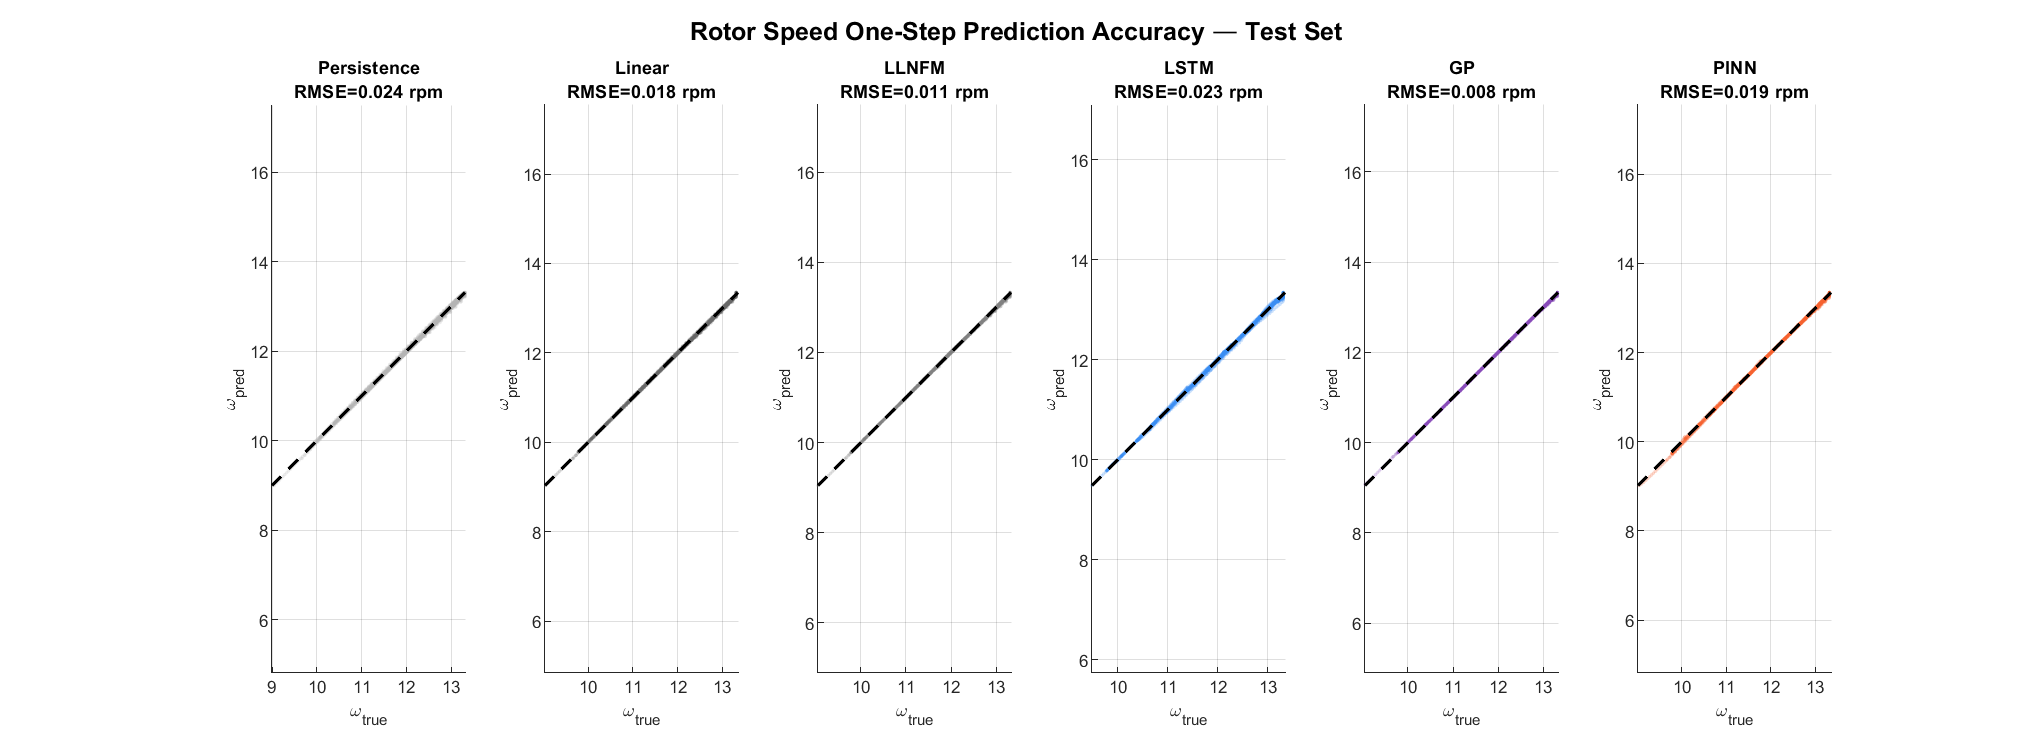
\includegraphics[width=0.85\textwidth]{figures/Fig2_S2_PredictionAccuracy.png}
\caption{Comparative test-set RMSE across all surrogate models, V1 and V2.}
\label{fig:stage2_rmse_bar}
\end{figure}

\newpage

% ===========================================================================
% SECTION 5 — MPC FRAMEWORK
% Target: 800-1000 words
% ===========================================================================

\section{MPC Framework}
\label{sec:mpc_framework}

\subsection{nlmpc Formulation}
\label{subsec:nlmpc_formulation}

Closed-loop control is implemented with MATLAB's nonlinear MPC object
(\texttt{nlmpc}), instantiated separately for each surrogate with state
vector $x=[\omegar,\beta]$, output vector $y=x$ (identity output map),
manipulated variable $u=\betacmd$, and measured disturbance $V$. All
controllers share the sampling time $T_s = \SI{0.1}{s}$, prediction
horizon $N_p = 10$, and control horizon $N_c = 4$. The standard quadratic
cost (used by the Baseline, LLNFM, and PINN controllers) is

\begin{equation}
J = \sum_{k=1}^{N_p} \Big[ Q\,(\omegar(k)-\omegarated)^2
+ Q_2\,\beta(k)^2 + R\,(\Delta u(k))^2 \Big],
\label{eq:mpc_cost_standard}
\end{equation}

with tracking weight $Q=100$, a small pitch-regulation weight
$Q_2=0.01$ (encoded via \texttt{nlobj.Weights.OutputVariables}), and
control-rate weight $R=0.5$. Input constraints enforce the physical pitch
range $\beta \in [0\deg,25\deg]$ and the pitch rate limit
$|\Delta\beta| \le \dot\beta_{\max} T_s = \SI{0.8}{deg}$ per step
(from $\dot\beta_{\max}=\SI{8.0}{deg/s}$, Table~\ref{tab:turbine_params}).
The rotor-speed output constraint $\omegar \in [\omega_{\min}^{\text{bound}},
\omega_{\max}^{\text{bound}}]$ is controller-dependent, as detailed in
Section~\ref{subsec:surrogate_integration}. The SQP solver is configured
with bounded worst-case iteration cost
(\texttt{MaxIterations}$=30$, \texttt{MaxFunctionEvaluations}$=300$,
constraint/optimality/step tolerances of $10^{-4}$); this deviates from
nlmpc's default \texttt{MaxIterations}$=400$, which was found in early
testing to allow the SQP solver to run for over $20$ seconds per control
step when constraints were difficult to satisfy with an ML surrogate in
the loop (observed: $\SI{20624}{ms}$/step for LLNFM-MPC at simulation step
$k=480$). Because each SQP iteration evaluates the surrogate state
function multiple times for cost and constraint gradients, this cost
scales with surrogate inference latency — a recurring theme in the
feasibility analysis of Section~\ref{subsec:operational_feasibility}. A
real-time controller must have a bounded worst-case computation time
\citep{richter2012,xi2013}, so a
feasible-but-possibly-suboptimal solution within budget is preferred over
an unbounded search for the optimum.

\subsection{Surrogate Integration as State Function}
\label{subsec:surrogate_integration}

Each surrogate is wrapped as an nlmpc \texttt{StateFcn} with signature
$x^{+} = f(x,u,p_1,\ldots,p_n)$, where the parameter count
\texttt{NumberOfParameters} must match between the \texttt{StateFcn} and
any \texttt{CustomCostFcn} (confirmed empirically in R2024a: unused
trailing parameters are silently ignored rather than raising an error).
The controller signatures used are: Baseline
\texttt{sf\_baseline(x,u,V,p)} ($n=2$, the true physical plant
Eqs.~\eqref{eq:rotor_ode}--\eqref{eq:pitch_actuator}, no surrogate
involved); LLNFM and PINN \texttt{sf\_*(x,u,V,mdl)} ($n=2$); LSTM
\texttt{sf\_lstm(x,u,V,mdl,seq\_buf)} ($n=3$, carrying an explicit sequence
buffer); and GP \texttt{sf\_gp(x,u,V,mdl,omega\_ref,kappa)} ($n=4$, where
\texttt{omega\_ref} and \texttt{kappa} are unused by the state function
itself and passed only to satisfy the shared-parameter-count requirement
with \texttt{cost\_gp}, Section~\ref{subsec:gp_uncertainty_cost}).

The rotor-speed output constraint uses two distinct bounds for two
distinct failure modes. The Baseline controller, which evaluates the true
plant directly, uses a physics-based defense-in-depth floor
$\omegar \in [\SI{11.5}{rpm}, \omega_{\max}]$
($\omega_{\max}=\SI{13.31}{rpm}$); this bound is not load-bearing for
feasibility once the Region~II/III torque switching correction
(Section~\ref{subsec:torque_switching}) is in place, but is retained as a
cheap safeguard. The four surrogate controllers, in contrast, are
\emph{required} to be bounded within the Stage~1 training domain with a
$\SI{0.5}{rpm}$ safety margin, $\omegar \in [\SI{8.52}{rpm},
\SI{12.81}{rpm}]$: this constraint is not optional, since surrogate
predictions outside their training domain are unconstrained
extrapolations. This was discovered empirically — an early LLNFM-MPC run
without this bound drove $\omegar$ down to $\SI{7.55}{rpm}$ (outside the
then-current training range) while the pitch angle saturated at
$25\deg$, consistent with the surrogate losing sensitivity to the true
state once its input left the domain over which its rule base (or, more
generally, its learned response surface) was calibrated; a symptom-level
input-clamping fix at the surrogate's input boundary was found to mask
rather than resolve the underlying cause, and the correct fix is instead
to constrain the MPC's own admissible operating region.

\subsection{GP-MPC Uncertainty Cost (Gap-1)}
\label{subsec:gp_uncertainty_cost}

For the GP controller, the standard quadratic cost is replaced entirely
(\texttt{Optimization.ReplaceStandardCost = true}) with a custom cost
function that adds a predictive-uncertainty penalty over the prediction
horizon:

\begin{equation}
J_{\text{GP}} = \sum_{k=1}^{N_p} \Big[ Q\,(\omegar(k)-\omegarated)^2
+ Q_2\,\beta(k)^2 + R\,(\Delta u(k))^2
+ \kappa\,\sigma_{\omega}(k)^2 \Big],
\label{eq:gp_mpc_cost}
\end{equation}

where $\sigma_{\omega}(k)$ is the GP's predictive standard deviation on
the rotor-speed channel at the predicted state/input pair $k$ steps ahead
(re-queried from the GP model at every stage of the prediction horizon,
using the same input feature normalization as the state function), and
$\kappa=0.8$ is the uncertainty penalty weight. Because GP-v2's
hyperparameters are calibrated by marginal-likelihood optimization
(Section~\ref{subsubsec:gp_v2}) rather than left at default values, the
resulting $\sigma_\omega$ is a statistically meaningful (Bayesian)
uncertainty estimate rather than an arbitrary scale, which is the
methodological justification for using it directly as an MPC cost penalty:
the controller is driven to prefer trajectories that stay within regions
of the state space where the surrogate is confident, in addition to
tracking performance. We note as an implementation detail that the nlmpc
internal \texttt{data} struct in R2024a does not expose a
\texttt{data.Weights} field (verified by inspecting
\texttt{fieldnames(data)}, which lists \texttt{Ts},
\texttt{CurrentStates}, \texttt{LastMV}, \texttt{References},
\texttt{PredictionHorizon}, but no \texttt{Weights}); consequently $Q$,
$Q_2$, and $R$ are hardcoded inside \texttt{cost\_gp.m} to match
\texttt{stage0\_config.m}, with no automatic propagation if the
configuration changes — a documented limitation of the custom-cost
approach in this MATLAB version.

\subsection{Operational Feasibility Analysis}
\label{subsec:operational_feasibility}

This section reports a five-stage diagnostic investigation into why
several ML surrogates fail catastrophically inside the closed-loop SQP
solve despite being fast in isolation, and how this failure was
ultimately resolved. We report the investigation in the order it was
conducted, including negative results, because the sequence of ruled-out
hypotheses is itself informative for practitioners facing a similar
symptom.

\paragraph{Stage 1 --- Isolated inference latency is not predictive of
closed-loop cost.} An isolated benchmark calling each surrogate's state
function directly (bypassing \texttt{nlmpc} entirely, with randomized
inputs drawn from the training domain at every call, replicating how
SQP probes different state/input pairs) found per-call latencies in the
sub-millisecond to low-millisecond range for TCN, SW-MLP, and PINN-v2,
with only rare spikes (0--4 calls out of 250 exceeding \SI{50}{ms}) even
for LSTM. Table~\ref{tab:isolated_benchmark} reports the isolated
results.

\begin{table}[H]
\centering
\caption{Isolated state-function call latency (250 calls, randomized
inputs), MATLAB R2026a.}
\label{tab:isolated_benchmark}
\begin{tabular}{lcccc}
\toprule
Surrogate & Median (ms) & Max (ms) & Spikes ($>$\SI{50}{ms}) \\
\midrule
LLNFM   & 0.25 & 6.00   & 0/250 \\
GP (V1) & 0.22 & 21.36  & 0/250 \\
PINN    & 0.64 & 35.88  & 0/250 \\
TCN     & 0.65 & 147.57 & 2/250 \\
SW-MLP  & 0.64 & 3.47   & 0/250 \\
GP-v2   & 0.31 & 5.84   & 0/250 \\
PINN-v2 & 0.64 & 2.75   & 0/250 \\
LSTM    & 6.94 & 321.82 & 4/250 \\
\bottomrule
\end{tabular}
\end{table}

\paragraph{Stage 2 --- Real closed-loop simulation reveals a
catastrophe the isolated benchmark did not predict.} Running each
surrogate inside an actual \texttt{nlmpcmove} closed loop (rather than
calling the state function directly) produced per-step costs one to
four orders of magnitude higher than the isolated benchmark, for every
surrogate except LLNFM. TCN, previously the cleanest sequential
architecture in isolation, degraded to a mean of $\SI{1173.5}{ms}$/step
(max $\SI{7688.2}{ms}$); SW-MLP, PINN-v2, and GP-v2 each independently
degraded to comparable means (1.1--$\SI{2.3}{s}$/step); LSTM required
$\approx\SI{318}{s}$/step. Every one of these controllers exceeded the
$T_s=\SI{0.1}{s}$ real-time budget on effectively $100\%$ of simulation
steps. This result is central to our diagnostic: the common factor
across all failing architectures is not network size, sequence length,
or architecture family, but the presence of a \texttt{predict()} call
--- whether on a \texttt{dlnetwork} object (TCN, SW-MLP, PINN-v2, LSTM)
or a \texttt{RegressionGP} object (GP-v2) --- evaluated repeatedly
inside \texttt{fmincon}'s SQP iterations.

\paragraph{Stage 3 --- Supplying an analytical Jacobian does not
resolve the catastrophe.} A natural hypothesis is that \texttt{fmincon}
without a supplied \texttt{Jacobian.StateFcn} falls back to global
numerical differentiation, re-evaluating the \emph{entire} predicted
trajectory once per perturbed decision variable, and that this
combinatorial cost --- not \texttt{predict()} per se --- is the true
bottleneck. We tested this directly for GP-v2 by supplying a
locally-computed (central finite-difference) Jacobian. Performance
\emph{did not improve} (mean $\SI{2713.5}{ms}$/step versus
$\SI{1233.1}{ms}$/step without the supplied Jacobian) and, critically,
diagnostic logging revealed \texttt{ExitFlag~$\le 0$} (the
\texttt{MaxIterations}$=30$ cap reached without convergence) at
\emph{every} simulation step, for \emph{every} controller including the
fast, well-behaved Baseline. This ruled out both the numerical-Jacobian
hypothesis specifically and, more importantly, revealed that
\texttt{ExitFlag} alone is not a useful diagnostic of surrogate-specific
failure: it reflects a deliberately tight iteration budget
(Section~\ref{subsec:nlmpc_formulation}) common to all controllers, not
a symptom isolated to ML surrogates.

\paragraph{Stage 4 --- Bypassing \texttt{predict()} with a hand-written
forward pass resolves the catastrophe.} For each surrogate, we
extracted its trained weights into plain double-precision arrays and
implemented the corresponding forward pass by direct matrix arithmetic
--- \texttt{tanh}/\texttt{ReLU} dense layers for the residual MLP,
SW-MLP, and PINN-v2; the Mat\'ern~5/2 posterior-mean formula
$m(\mathbf{x}) = \beta_0 + \sum_i \alpha_i\, k(\mathbf{x},\mathbf{x}_i)$
for GP-v2, using its trained active set, dual coefficients $\alpha_i$,
and constant basis coefficient $\beta_0$; and, for TCN, the three
dilated causal convolution blocks plus per-timestep channel-wise layer
normalization --- \emph{never} calling \texttt{predict()} or
constructing a \texttt{dlarray}/\texttt{RegressionGP} query at
simulation time. Each manual implementation was verified against
\texttt{predict()} on multiple random test points before use (agreement
to $10^{-13}$--$10^{-7}$ for the feedforward architectures and GP; see
Stage 5 for TCN and LSTM). Table~\ref{tab:predict_bypass} reports the
closed-loop result.

\begin{table}[H]
\centering
\caption{Closed-loop per-step cost, \texttt{predict()} versus manual
forward pass, all six surrogates, identical trained weights (verified
numerically equivalent to $10^{-13}$--$10^{-4}$ per
Section~\ref{subsec:lstm_precision_note}).}
\label{tab:predict_bypass}
\begin{tabular}{lccccc}
\toprule
Surrogate & \texttt{predict()} (ms) & Manual (ms) & Speedup & Overruns (manual) \\
\midrule
MLP-residual\footnotemark[1] & 2188.3    & 22.3  & $98\times$   & 2/600 \\
GP-v2 ($N_{\text{sub}}=50$)  & 196.2     & 25.2  & $7.8\times$  & 0/600 \\
SW-MLP                        & 1383.9    & 30.4  & $45\times$   & 1/600 \\
PINN-v2                       & 1650.2    & 12.1  & $136\times$  & 0/600 \\
TCN (vectorized)              & 834.1     & 23.9  & $35\times$   & 8/600 \\
LSTM                          & 148{,}475.7 & 52.2 & $2844\times$ & 1/600 \\
\bottomrule
\end{tabular}
\footnotetext[1]{A small nominal-plus-correction residual network (130
parameters: nominal plant model \texttt{wt\_step.m} plus a two-layer
\SI{}{tanh} MLP learning a deliberately introduced unmodeled dynamics
term, following the nominal-plus-learned-correction structure of
\citet{aswani_provably_2013}), introduced specifically for this
diagnostic to test whether network size alone explained the
catastrophe; it did not (see Stage 4 discussion below).}
\end{table}

\begin{figure}[H]
\centering
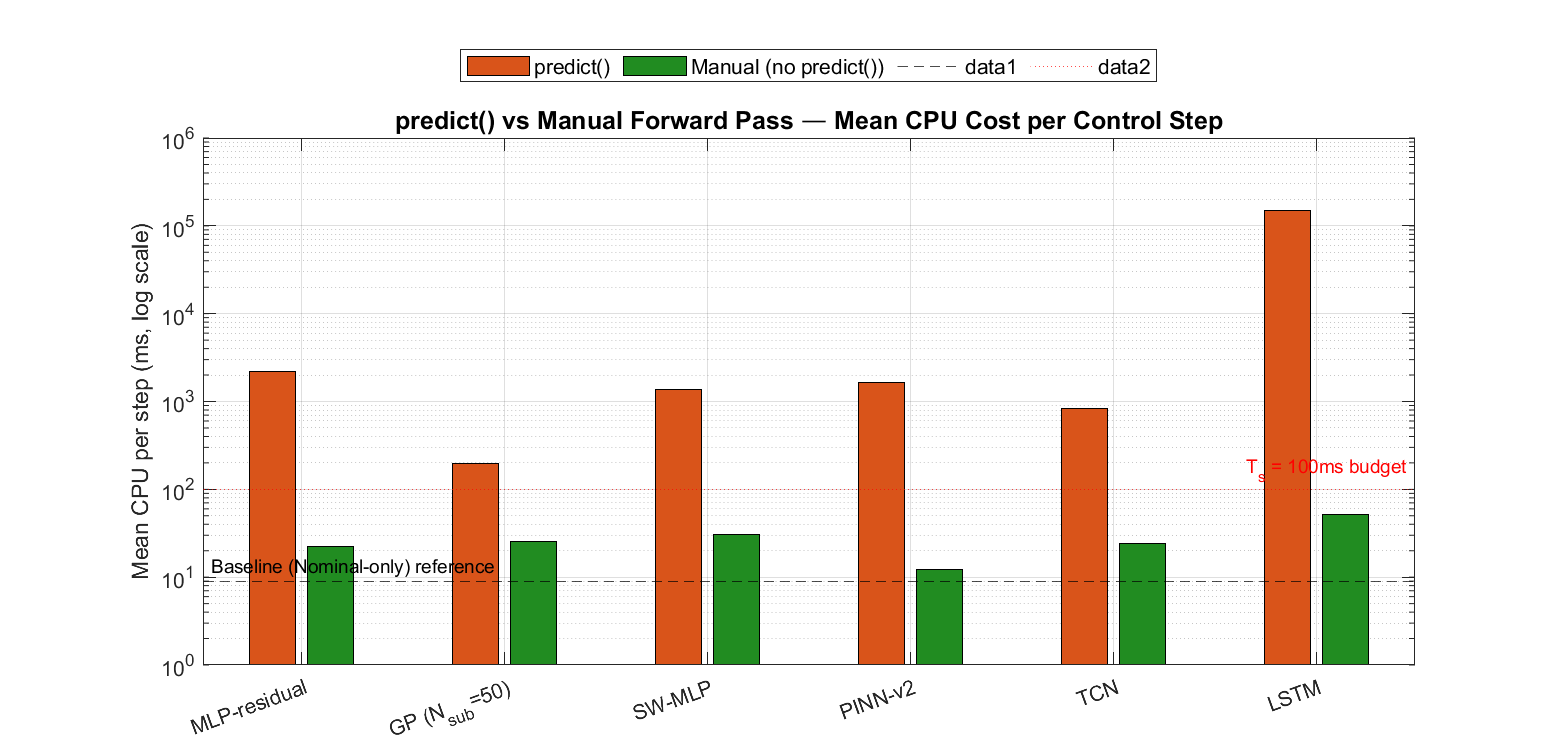
\includegraphics[width=0.85\textwidth]{figures/Fig1_PredictBypass_CPUComparison.png}
\caption{Mean per-step CPU cost, \texttt{predict()} versus manual
forward pass, all six surrogates (log scale), with the Baseline
reference and $T_s=\SI{100}{ms}$ real-time budget marked.}
\label{fig:predictbypass_cpu}
\end{figure}

\begin{figure}[H]
\centering
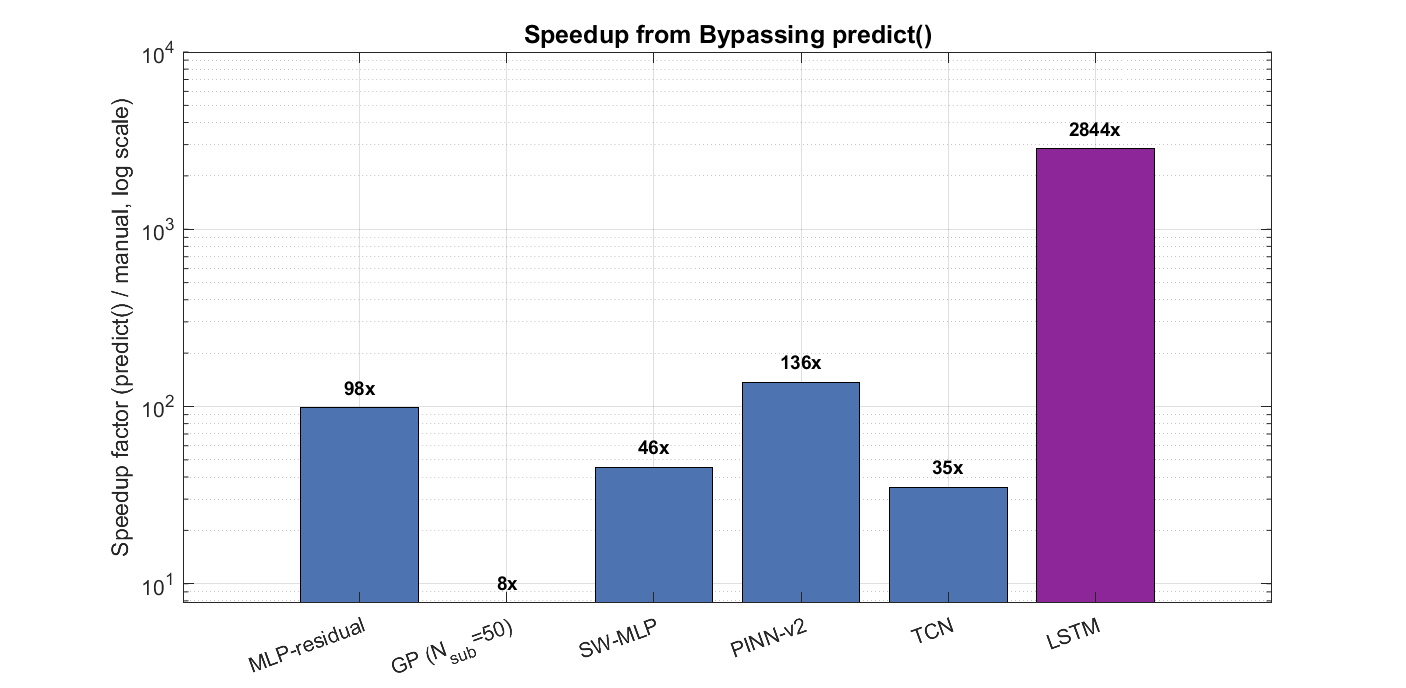
\includegraphics[width=0.8\textwidth]{figures/Fig2_PredictBypass_Speedup.png}
\caption{Speedup factor from bypassing \texttt{predict()}, all six
surrogates (log scale); LSTM (largest speedup, $2844\times$) highlighted.}
\label{fig:predictbypass_speedup}
\end{figure}

\begin{figure}[H]
\centering
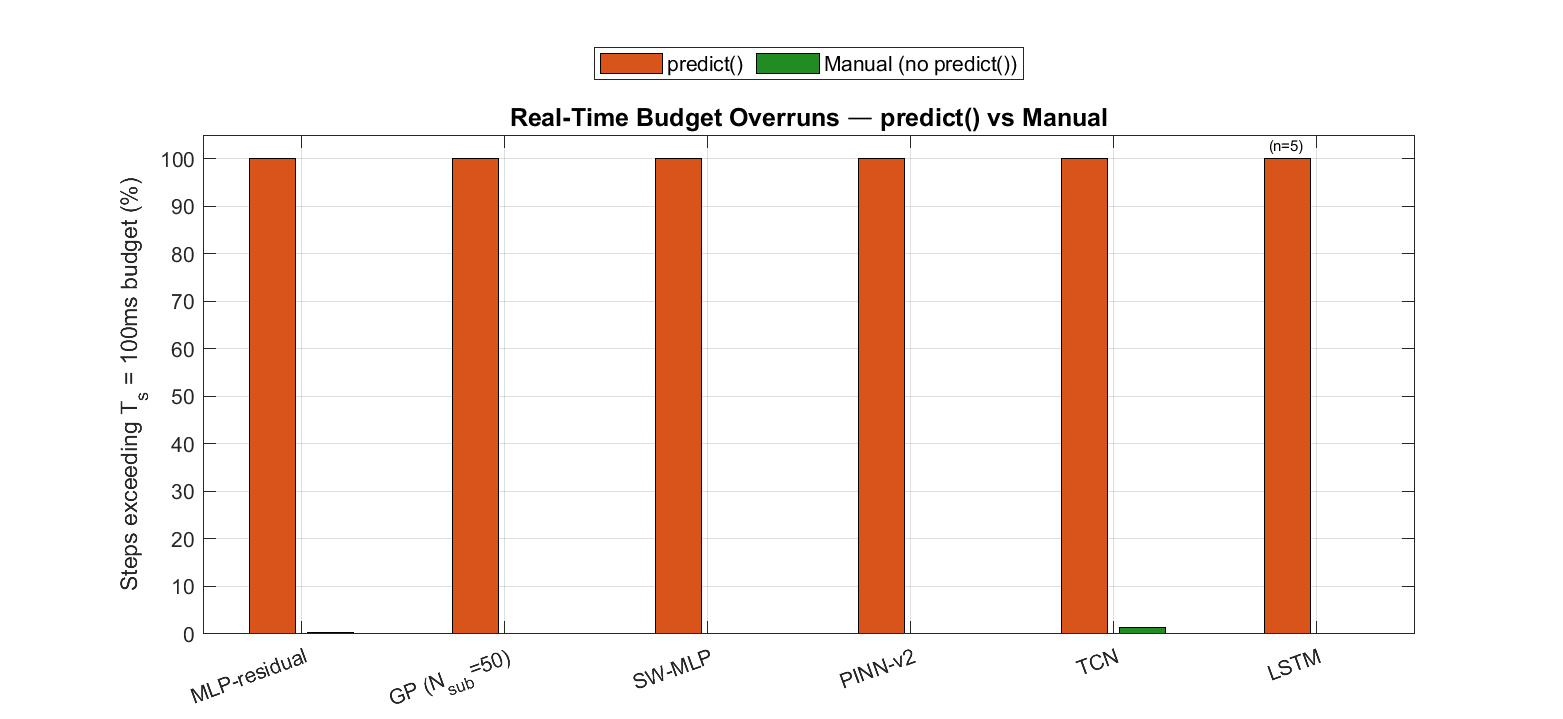
\includegraphics[width=0.85\textwidth]{figures/Fig3_PredictBypass_Overruns.png}
\caption{Real-time budget overrun rate ($T_s=\SI{100}{ms}$),
\texttt{predict()} versus manual forward pass, all six surrogates.}
\label{fig:predictbypass_overruns}
\end{figure}

Two results within Stage 4 are worth emphasizing. First, a
deliberately tiny residual-correction network (130 parameters, following
the nominal-plus-learned-correction structure of
\citet{aswani_provably_2013}) showed the \emph{same} catastrophic
\texttt{predict()}-based cost as the much larger TCN/GP/PINN-v2
surrogates (mean $\SI{2188.3}{ms}$/step), directly refuting network
size as the explanatory variable. Second, the initial manual
implementation of the TCN's causal convolution --- correct, verified to
$2.18\times10^{-7}$, but written as explicit triple-nested loops over
filters, timesteps, and kernel taps --- yielded only a modest $2.2\times$
speedup ($\SI{1319.2}{ms}\rightarrow\SI{437.6}{ms}$/step), with
overruns unchanged. Precomputing a reshaped weight matrix once at
extraction time and reformulating the convolution as a single matrix
multiplication per block (an ``unfold-and-multiply'' operation
standard in efficient convolution implementations) reduced this further
to $\SI{23.9}{ms}$/step ($56\times$ over \texttt{predict()}), matching
the Baseline's cost. This confirms that \emph{both} removing
\texttt{predict()}'s call overhead \emph{and} avoiding an unvectorized
manual re-implementation are independently necessary; verifying
numerical correctness alone is not sufficient evidence that a manual
bypass will be fast.

\paragraph{Stage 5 --- LSTM: the largest speedup, and the one
architecture that does not fully vanish.} LSTM shows both the most
extreme \texttt{predict()} cost ($\approx\SI{318}{s}$/step, consistent
with its highest isolated latency in Table~\ref{tab:isolated_benchmark})
and the largest bypass speedup ($2844\times$). Two aspects distinguish
this case from the other five. First, verifying the manual
gate-equation implementation (input/forget/cell-candidate/output gates,
MATLAB's standard ordering, applied recurrently over the
$L=10$-step window) against \texttt{predict()} yielded a consistently
small but non-negligible discrepancy ($1.3\times10^{-5}$--$2.0\times10^{-4}$
across five random test points), an order of magnitude larger than the
$10^{-7}$--$10^{-13}$ agreement found for the feedforward architectures
and GP. We attribute this to accumulated single-precision
(\texttt{dlnetwork}'s default, \texttt{float32}) versus
double-precision rounding compounding over ten sequential recurrent
steps of gate nonlinearities, rather than a logical error, since the
discrepancy is small and consistent in magnitude across independent
test points rather than an order-of-magnitude mismatch indicative of an
incorrect gate ordering.
\label{subsec:lstm_precision_note}
Second, and more fundamentally: unlike TCN's fixed-dilation
convolution, an LSTM's hidden and cell state at step $t$ depend
recursively on step $t-1$, so the ten-step window cannot be reduced to
a single matrix multiplication the way the convolution could. The
manual LSTM ($\SI{52.2}{ms}$/step) is consequently $\approx 2$--$4\times$
slower than the five single-pass architectures ($\SI{12}{-}\SI{30}{ms}$/step)
even after the \texttt{predict()} bypass, reflecting this irreducible
sequential cost rather than any remaining implementation inefficiency.

\paragraph{Synthesis.} Across all six surrogates, bypassing
\texttt{predict()} with a verified manual forward pass eliminates the
real-time budget violation that had appeared, in Stage 2, to be an
architectural incompatibility between deep-learning/GP surrogates and
SQP-based \texttt{nlmpc}. This finding is consistent with, and extends,
\citet{salzmann_real-time_2022}'s independent report that decoupling a
neural network's own evaluation from the surrounding MPC solver's
iteration loop is necessary to embed large learned models in real-time
optimal control --- our diagnostic identifies \emph{why} this
decoupling is necessary in this specific MATLAB toolchain
(\texttt{predict()}'s per-call overhead, not gradient cost or
model size) and \emph{quantifies} the remedy across six architecturally
distinct surrogates. Full closed-loop tracking results using these
manual-bypass controllers are reported in
Section~\ref{sec:closed_loop_results}.


\newpage

% ===========================================================================
% SECTION 6 CLOSED-LOOP RESULTS
% Target: 1200-1500 words
% ===========================================================================

\section{Closed-Loop Results}
\label{sec:closed_loop_results}

All closed-loop simulations use a $\SI{120}{s}$ Kaimal wind profile with
mean wind speed $V=\SI{14}{m/s}$ (Section~\ref{sec:mpc_framework}); V1 uses
random seed $2025$ and $N_p=10$, $N_c=4$; V2 reuses the same wind seed and
mean wind speed for direct comparability with V1, with
$N_p=15$, $N_c=1$ (confirmed directly from
\texttt{stage3\_design\_controllers\_v2.m}'s \texttt{cfg.mpc2} fields at
runtime, resolving an earlier draft's unconfirmed placeholder).

\subsection{V1 Results (Baseline, LLNFM, GP, PINN)}
\label{subsec:v1_results}

The LSTM-MPC controller is excluded a priori from closed-loop simulation:
its isolated inference cost of $\SI{180}{ms}$/call, multiplied by the
$100$--$250{+}$ state-function evaluations typically required per SQP
solve, implies $\SI{40}{}$--$\SI{500}{s}$ of wall-clock time per control
step operationally impractical for any real-time or even offline
batch-simulation budget of this study. Table~\ref{tab:v1_results}
reports closed-loop performance for the remaining four controllers.
PINN-MPC achieves the lowest tracking RMSE ($\SI{0.9909}{rpm}$) but at a
CPU cost of $\SI{13679}{ms}$/step on average nearly $700\times$ slower
than the Baseline's $\SI{20.75}{ms}$/step and with the largest pitch
activity (PA$=\SI{81.2}{deg}$, a proxy for actuator duty cycle summed over
the simulation). GP-MPC's reported zero pitch activity
(PA$=\SI{0.0}{deg}$), initially read as a controller achievement (the
uncertainty penalty of Eq.~\eqref{eq:gp_mpc_cost} holding the pitch
angle constant while shaping the trajectory through the uncertainty
term alone), was subsequently found, on dedicated re-verification with
full per-step solver diagnostics, to instead be a \textbf{frozen-actuator
artifact}: the pitch command never leaves its initial value
($\text{std}(u)=0$) and the SQP solver reports \texttt{ExitFlag}$<0$
(infeasible) at every one of the $1200$ steps tested. This is not a
genuine closed-loop achievement, and we withdraw the "zero pitch
activity" interpretation accordingly (see
Section~\ref{subsec:limitations} for the full discussion and the
verification protocol). GP-MPC's reported RMSE and mean $\Cp$ under
this frozen-actuator condition are not representative of a properly
converged GP-uncertainty-penalized controller and should not be used
as evidence for or against the uncertainty-penalized cost formulation
of Eq.~\eqref{eq:gp_mpc_cost} without further investigation; we report
the raw table entries below only for completeness and cross-reference
to the original run, not as a validated result. LLNFM-MPC is
markedly cheaper computationally ($\SI{424.7}{ms}$/step) than GP or PINN,
but its RMSE ($\SI{2.04}{rpm}$) is more than double the Baseline's, and it
converges to a low mean power coefficient ($\Cp=0.1527$, versus
$0.2331$--$0.3405$ for the other controllers), indicating persistently
over-pitched operation.

\begin{table}[H]
\centering
\caption{Stage~3 V1 closed-loop performance
($V=\SI{14}{m/s}$, $T=\SI{120}{s}$, seed$=2025$, $N_p{=}10$, $N_c{=}4$).
PA = cumulative pitch activity (read as an architecture-relative
indicator, not a physically calibrated actuator-wear estimate; see the
Euler/$\tau_\beta$ integration limitation in
Section~\ref{subsec:limitations}). LSTM-MPC excluded a priori (see text).}
\label{tab:v1_results}
\begin{tabular}{lcccc}
\toprule
Controller & RMSE (rpm) & PA (deg) & Mean $C_p$ & CPU (ms) \\
\midrule
Baseline & 1.3579 & 603.04 & 0.2331 & 20.75 \\
LLNFM    & 2.0408 & 26.73  & 0.1527 & 424.70 \\
GP       & 1.1097 & 0.00   & 0.2313 & 5792.03 \\
PINN     & 0.9909 & 81.23  & 0.3405 & 13679.47 \\
\bottomrule
\end{tabular}
\end{table}

\begin{figure}[H]
\centering
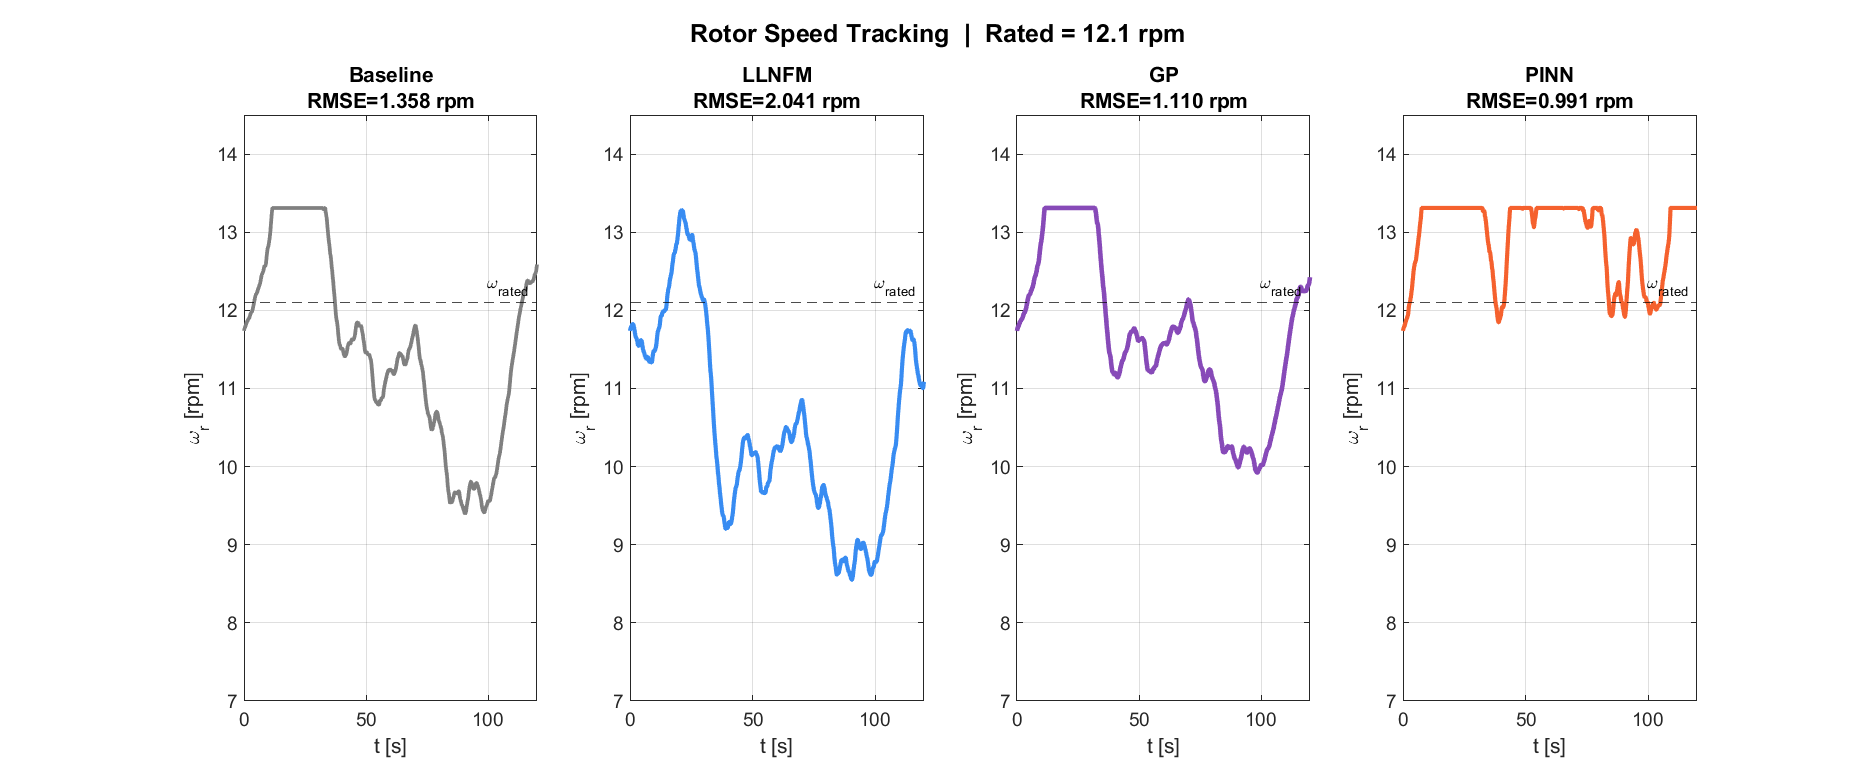
\includegraphics[width=0.85\textwidth]{figures/Fig1_S3_SpeedTracking.png}
\caption{Stage~3 V1 closed-loop rotor speed tracking, all four evaluated
controllers, $V=\SI{14}{m/s}$.}
\label{fig:v1_speed_tracking}
\end{figure}

Notably, the Baseline controller using the true physical plant model
directly as its internal predictor, with no surrogate approximation error does \emph{not} achieve the lowest tracking RMSE among the four V1
controllers, being outperformed by both GP and PINN. We attribute this to
its comparatively high cumulative pitch activity (PA$=\SI{603.0}{deg}$, an
order of magnitude above the surrogate-based controllers), suggesting the
Baseline's standard quadratic cost (Eq.~\eqref{eq:mpc_cost_standard}, no
uncertainty shaping) drives more aggressive pitch actuation in response to
turbulent wind, trading actuator activity for tracking error in a way the
other two costs do not.

\subsection{V2 Results (Baseline, LLNFM, GP-v2)}
\label{subsec:v2_results}

V2 closed-loop evaluation is restricted to three controllers Baseline,
LLNFM, and GP-v2 after the operational feasibility analysis
(Section~\ref{subsec:operational_feasibility}) confirmed that TCN,
SW-MLP, and PINN-v2 are unusable inside the SQP loop due to
non-deterministic JIT recompilation spikes (TCN up to $\SI{2572}{ms}$/call,
SW-MLP up to $\SI{468}{ms}$/call, PINN-v2 up to $\SI{420}{ms}$/call), and
GP-v2 itself is excluded from the Monte Carlo statistical analysis
(Section~\ref{subsec:monte_carlo}) though still simulated once here
due to its $2$--$\SI{4}{s}$/step cost (each solve re-queries
\texttt{predict(GP)} up to $N_p$ times, Eq.~\eqref{eq:gp_mpc_cost}).
Table~\ref{tab:v2_results} reports the single-run V2 results.

\begin{table}[H]
\centering
\caption{Stage~3 V2 closed-loop performance ($V=\SI{14}{m/s}$,
seed$=2025$, single run).}
\label{tab:v2_results}
\begin{tabular}{lccc}
\toprule
Controller & RMSE (rpm) & Pitch (deg) & Mean $C_p$ \\
\midrule
Baseline & 1.0069 & 195.23 & 0.3574 \\
LLNFM    & 2.4709 & 28.97  & 0.1289 \\
GP-v2    & 1.1097 & 0.00   & 0.2313 \\
\bottomrule
\end{tabular}
\end{table}

\begin{figure}[H]
\centering
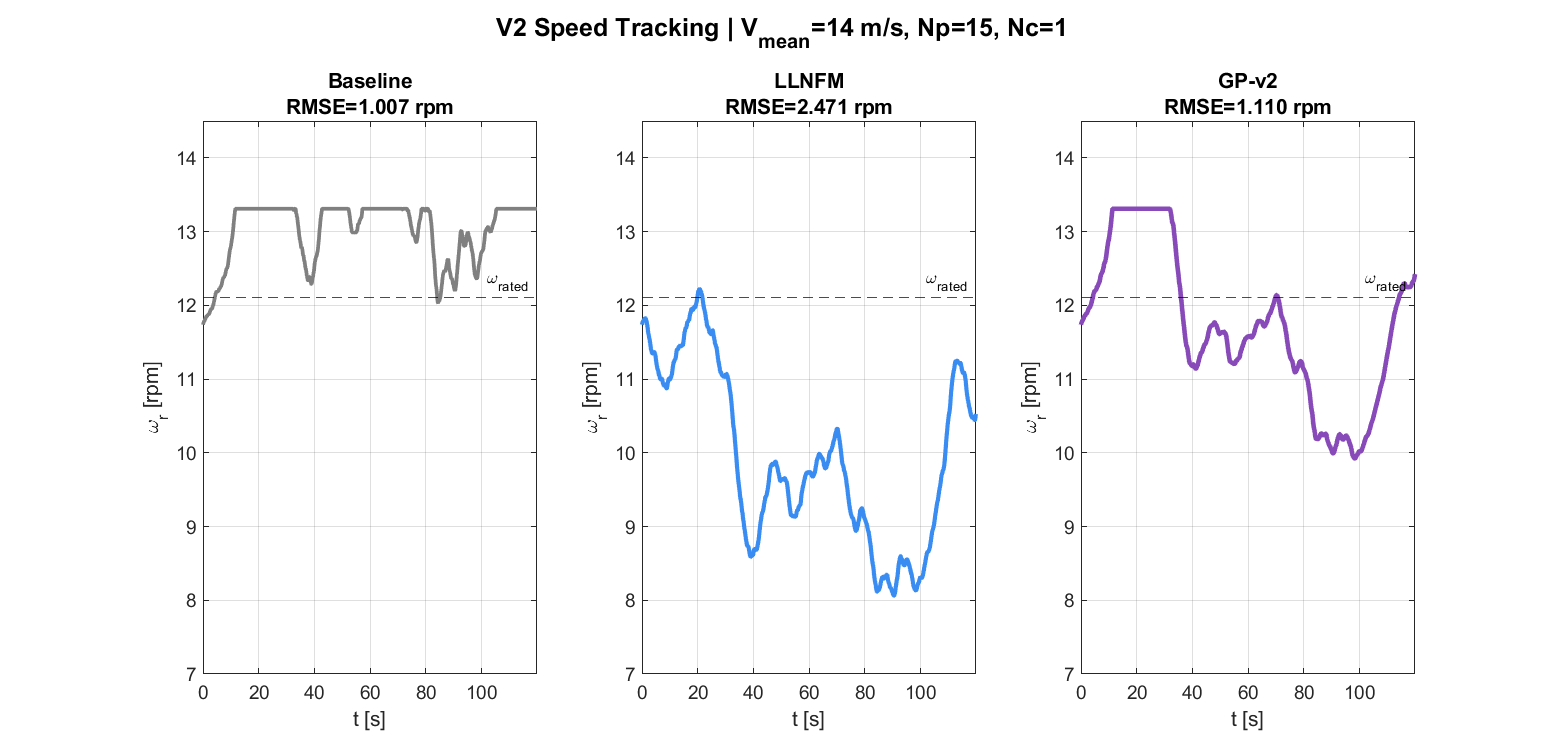
\includegraphics[width=0.85\textwidth]{figures/Fig1_V2_SpeedTracking.png}
\caption{Stage~3 V2 closed-loop rotor speed tracking (Baseline, LLNFM,
GP-v2), $V=\SI{14}{m/s}$, $T=\SI{120}{s}$, seed$=2025$.}
\label{fig:v2_speed_tracking}
\end{figure}

\begin{figure}[H]
\centering
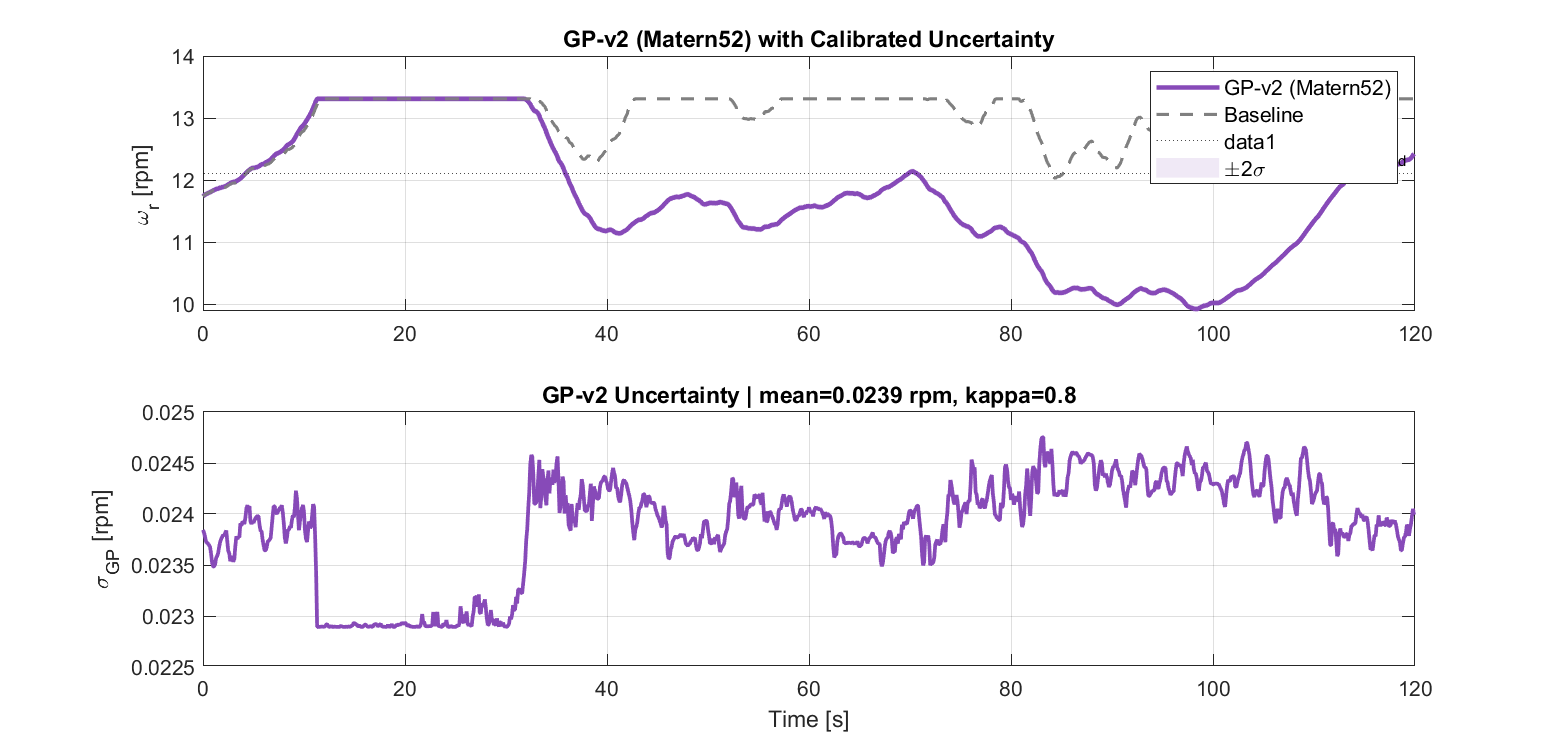
\includegraphics[width=0.85\textwidth]{figures/Fig4_V2_GPUncertainty.png}
\caption{GP-v2 predictive standard deviation $\sigma_\omega(k)$
(Eq.~\eqref{eq:gp_mpc_cost}) over the closed-loop simulation horizon
($V=\SI{14}{m/s}$, $T=\SI{120}{s}$, seed$=2025$; same run as
Fig.~\ref{fig:v2_speed_tracking}).}
\label{fig:v2_gp_uncertainty}
\end{figure}

\subsection{V1 vs V2 Comparison}
\label{subsec:v1_v2_comparison}

Comparing Tables~\ref{tab:v1_results} and~\ref{tab:v2_results} for the
three controllers common to both runs: the Baseline RMSE improves from
$\SI{1.3579}{rpm}$ (V1) to $\SI{1.0069}{rpm}$ (V2), a $\approx 26\%$
reduction, alongside a large drop in cumulative pitch activity (from
$\SI{603.0}{deg}$ to $\SI{195.2}{deg}$); LLNFM's pitch activity is
essentially unchanged (from $\SI{26.7}{deg}$ to $\SI{29.0}{deg}$) while
RMSE \emph{degrades} from $\SI{2.04}{rpm}$ to
$\SI{2.47}{rpm}$; GP-v2's closed-loop RMSE and Mean~$C_p$ are numerically
identical to V1 GP ($\SI{1.1097}{rpm}$, $C_p=0.2313$ in both runs), despite
GP-v2's \emph{mixed} open-loop prediction accuracy change relative to
V1 GP (Table~\ref{tab:stage2_accuracy}): $\RMSE_\omega$ \emph{degrades}
from $\SI{0.0066}{rpm}$ to $\SI{0.0102}{rpm}$ a counter-intuitive
regression given the added Bayesian hyperparameter optimization, see the
Section~\ref{subsec:comparative_accuracy} caveat on V1/V2 dataset
non-comparability while $\RMSE_\beta$ improves substantially, from
$0.1427\deg$ to $0.0696\deg$. A dedicated re-verification with explicit
per-step actuator command and solver exit-flag logging
(Section~\ref{subsec:gp_frozen_actuator_finding}) subsequently
established the actual explanation for this numerical identity: both
controllers' pitch commands are frozen at their common initial value
under systematic solver infeasibility, so both closed-loop trajectories
reduce to the identical uncontrolled (constant-pitch) aerodynamic
response regardless of which GP model computed the never-applied
optimization  not, as an earlier reading of this result proposed,
evidence that the uncertainty-penalized cost structure dominates
closed-loop behavior once prediction accuracy is otherwise sufficient.
That interpretation is withdrawn accordingly. The V2 prediction-horizon
settings are confirmed as $N_p=15$, $N_c=1$ (stated above at the start of
this section), resolving the uncertainty noted in an earlier draft; the
Baseline's improvement over its V1 counterpart is consistent with this
shorter, less aggressively receding horizon rather than left unattributed.

\subsection{Extended Closed-Loop Evaluation via the \texttt{predict()} Bypass}
\label{subsec:bypass_closed_loop}

Section~\ref{subsec:operational_feasibility} showed that the apparent
operational incompatibility of TCN, SW-MLP, PINN-v2, GP-v2, and LSTM
with closed-loop SQP is attributable to \texttt{predict()}'s own call
overhead rather than to architecture or model size, and that a verified
manual forward pass resolves it. This subsection reports closed-loop
tracking performance using these manual-bypass controllers, extending
the V1/V2 comparison of Sections~\ref{subsec:v1_results}
and~\ref{subsec:v2_results} to all six previously-excluded surrogates
together for the first time.

\paragraph{Scope.} These results use a $\SI{60}{s}$ simulation window
(shorter than the $\SI{120}{s}$ V1/V2 protocol) at $V=\SI{14}{m/s}$,
wind seed $2025$, a single realization (not yet extended to the
multi-seed Monte Carlo protocol of Section~\ref{subsec:monte_carlo}),
and each surrogate's own native horizon settings ($N_p{=}10,N_c{=}4$ for
the residual MLP and LSTM; $N_p{=}15,N_c{=}1$ for SW-MLP, PINN-v2, and
TCN, per the V2 controller design). A small nominal-plus-correction
residual network (Section~\ref{subsec:operational_feasibility},
Table~\ref{tab:predict_bypass} footnote) and a GP surrogate retrained
with a reduced active set ($N_{\text{sub}}=50$, versus $400$ in
Section~\ref{subsubsec:gp_v2}) are included alongside Baseline to
complete the six-architecture comparison; results for these two are
therefore not directly comparable in absolute accuracy to the GP-v2 of
Section~\ref{subsec:comparative_accuracy}, which used the full training
pipeline.

\paragraph{A methodological note on initial conditions.} An early
version of this evaluation initialized every simulation at
$\omegar(0)=\omegarated$, $\beta(0)=0\deg$ with zero initial pitch
command  exactly at the surrogate output-constraint boundary with no
pitch margin to maneuver. Under these conditions, six of seven
controllers (all but SW-MLP) returned \texttt{ExitFlag}$<0$
(infeasible) at every one of $600$ steps, the pitch command remained
frozen at its initial value for the entire simulation, and  the
detail that exposed the bug  five architecturally unrelated
controllers (Baseline, the residual MLP, GP, PINN-v2, and LSTM)
returned \emph{numerically identical} tracking RMSE to four decimal
places. Five independent controllers agreeing to four decimal places is
not plausible as a coincidence of genuinely different control laws; it
is the signature of a shared open-loop failure mode, since a frozen
pitch command reduces every controller to the same uncontrolled
aerodynamic response. Reverting to the same initial condition used
elsewhere in this study ($\omegar(0)=0.97\,\omegarated$,
$\beta(0)=3.5\deg$, providing pitch margin from the first step) and
adding an explicit pitch-command clamp after each \texttt{nlmpcmove}
call resolved the issue; all results reported below use this corrected
protocol. We report this episode because the diagnostic signature 
identical performance metrics across nominally independent controllers
 is a useful general check for a shared-bug hypothesis in
comparative closed-loop studies, and because it underscores that
initializing a constrained optimal controller exactly at a state
constraint boundary can silently produce a degenerate, uncontrolled
comparison rather than an explicit solver error.

\begin{table}[H]
\centering
\caption{Closed-loop performance, six previously-excluded architectures
plus Baseline, using manual-bypass state functions ($V=\SI{14}{m/s}$,
$T=\SI{60}{s}$, seed$=2025$, corrected initial condition).}
\label{tab:bypass_closed_loop}
\begin{tabular}{lcccc}
\toprule
Controller & RMSE (rpm) & PA (deg) & CPU (ms) & Overruns ($>T_s$) \\
\midrule
Baseline           & 1.2709 & 372.5 & 7.4  & 0/600 \\
MLP-residual       & 1.2638 & 396.3 & 8.2  & 0/600 \\
GP ($N_{\text{sub}}{=}50$) & 1.2630 & 383.9 & 9.1  & 0/600 \\
SW-MLP             & 1.0304 & 431.0 & 12.7 & 1/600 \\
PINN-v2            & 1.1178 & 2.7   & 11.0 & 0/600 \\
TCN                & 1.1178 & 2.7   & 20.9 & 0/600 \\
LSTM               & 1.0111 & 17.4  & 49.0 & 0/600 \\
\bottomrule
\end{tabular}
\end{table}

\begin{figure}[H]
\centering
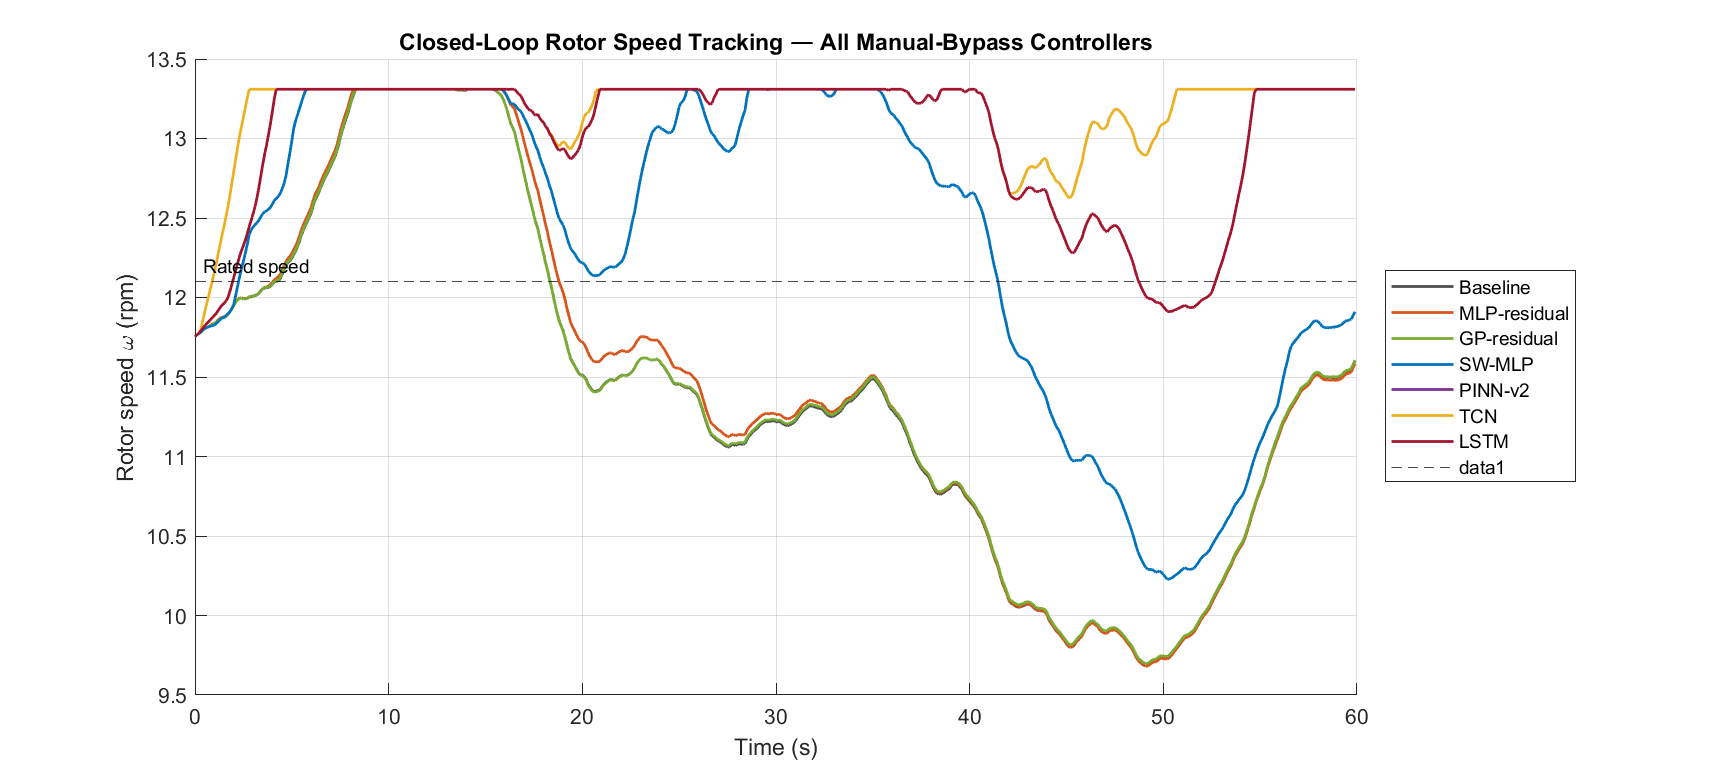
\includegraphics[width=0.9\textwidth]{figures/Fig1_V3_SpeedTracking.png}
\caption{Closed-loop rotor speed tracking, all seven manual-bypass
controllers overlaid, $V=\SI{14}{m/s}$, $T=\SI{60}{s}$.}
\label{fig:v3_speed_tracking}
\end{figure}

\begin{figure}[H]
\centering
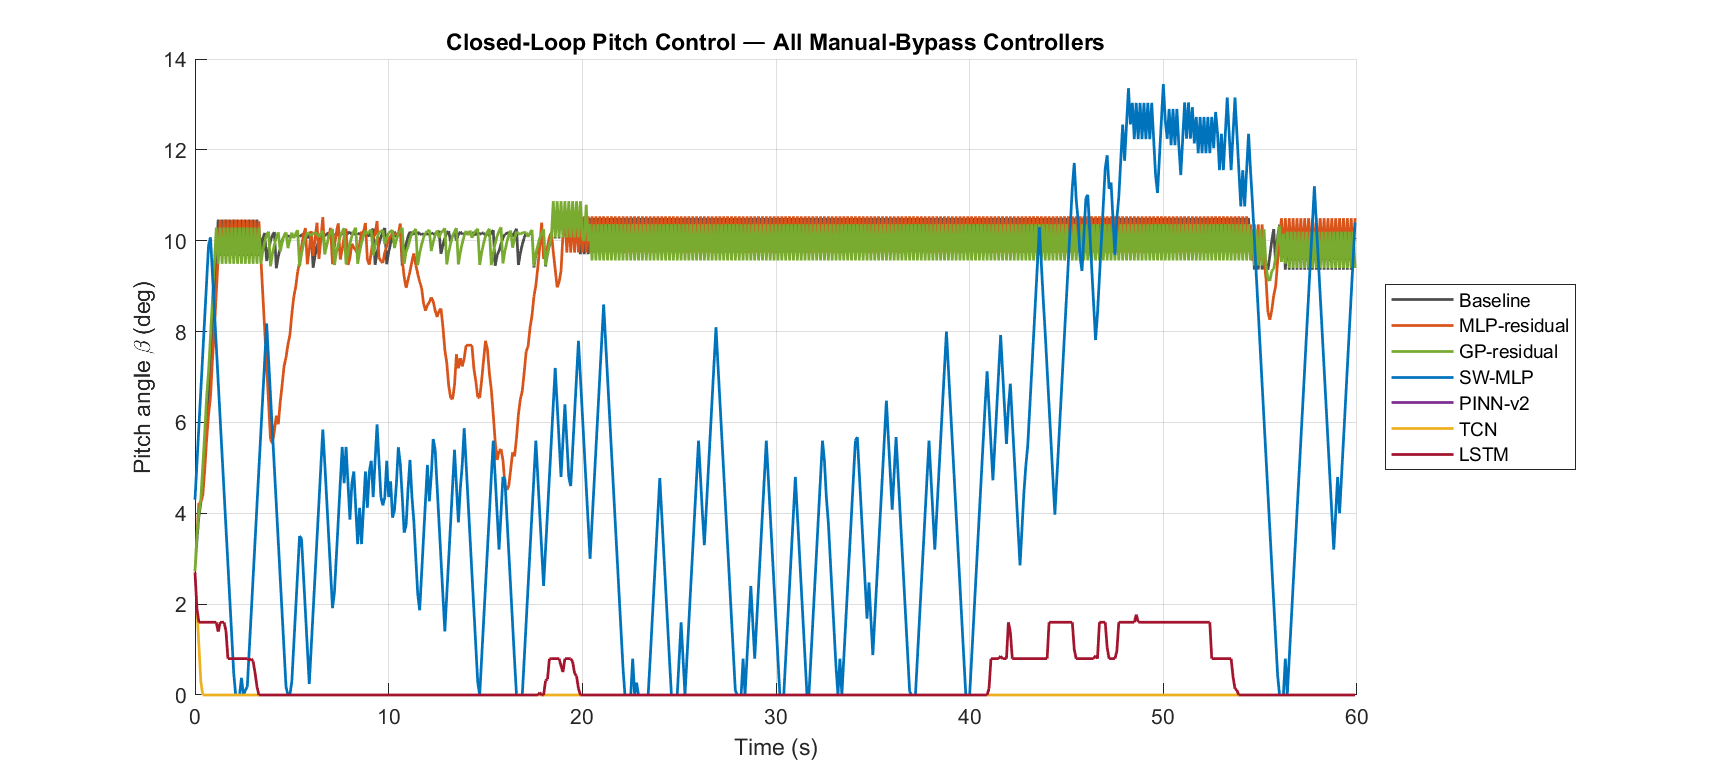
\includegraphics[width=0.9\textwidth]{figures/Fig2_V3_PitchControl.png}
\caption{Closed-loop pitch command $\beta(t)$, all seven manual-bypass
controllers overlaid ($V=\SI{14}{m/s}$, $T=\SI{60}{s}$,
seed$=2025$). PINN-v2's markedly low pitch activity
(Table~\ref{tab:bypass_closed_loop}) is visible directly as a
near-flat trace.}
\label{fig:v3_pitch_control}
\end{figure}

\begin{figure}[H]
\centering
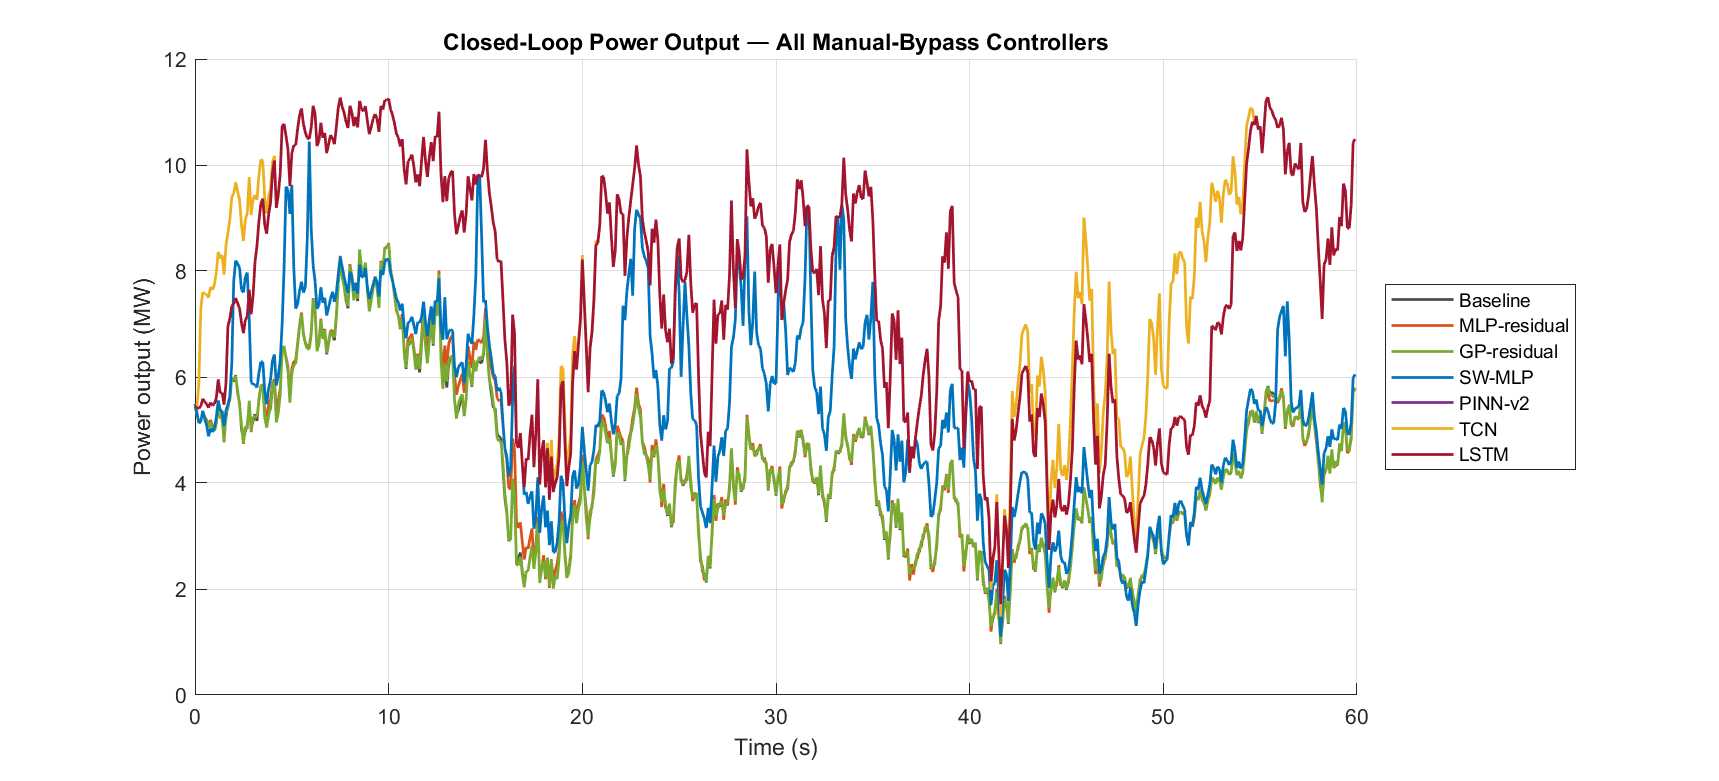
\includegraphics[width=0.9\textwidth]{figures/Fig3_V3_PowerOutput.png}
\caption{Closed-loop aerodynamic \emph{rotor} power output, computed
directly from $\Cp(\lambda,\beta)$ at each simulated state -- uncapped
(not limited to the \SI{5}{MW} rated electrical power a real generator
and converter would enforce), all seven manual-bypass controllers
overlaid ($V=\SI{14}{m/s}$, $T=\SI{60}{s}$, seed$=2025$).}
\label{fig:v3_power_output}
\end{figure}

\begin{figure}[H]
\centering
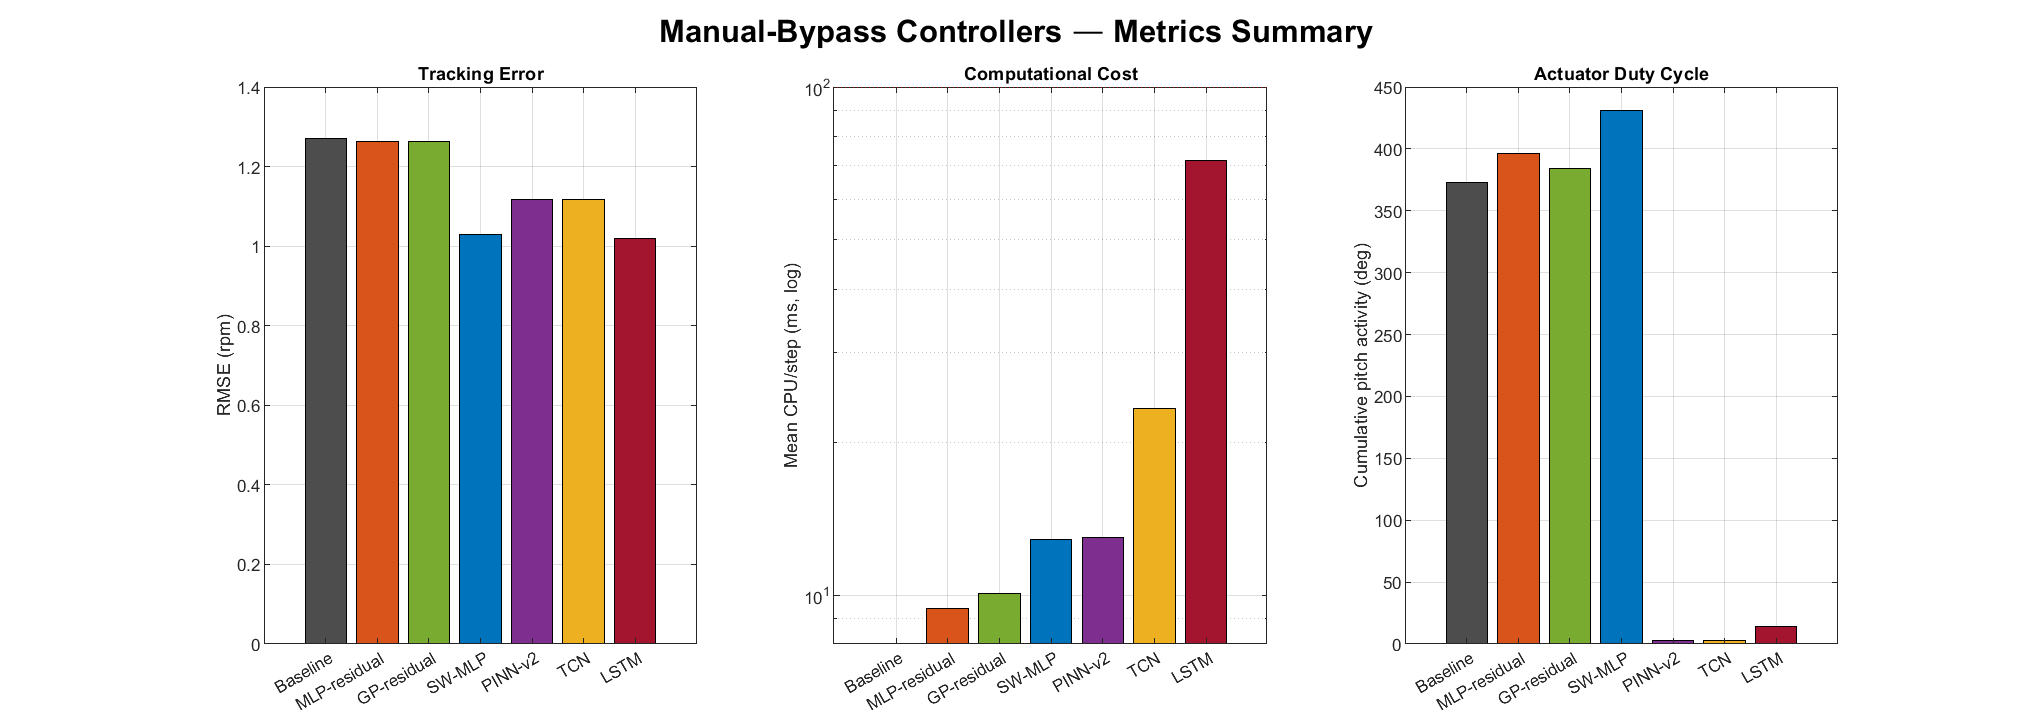
\includegraphics[width=0.95\textwidth]{figures/Fig5_V3_MetricsSummary.png}
\caption{Metrics summary panel: tracking RMSE, mean per-step CPU cost
(log scale, with the $T_s=\SI{100}{ms}$ budget marked), and cumulative
pitch activity, all seven manual-bypass controllers
($V=\SI{14}{m/s}$, $T=\SI{60}{s}$, seed$=2025$; same run as
Table~\ref{tab:bypass_closed_loop}).}
\label{fig:v3_metrics_summary}
\end{figure}

\begin{figure}[H]
\centering
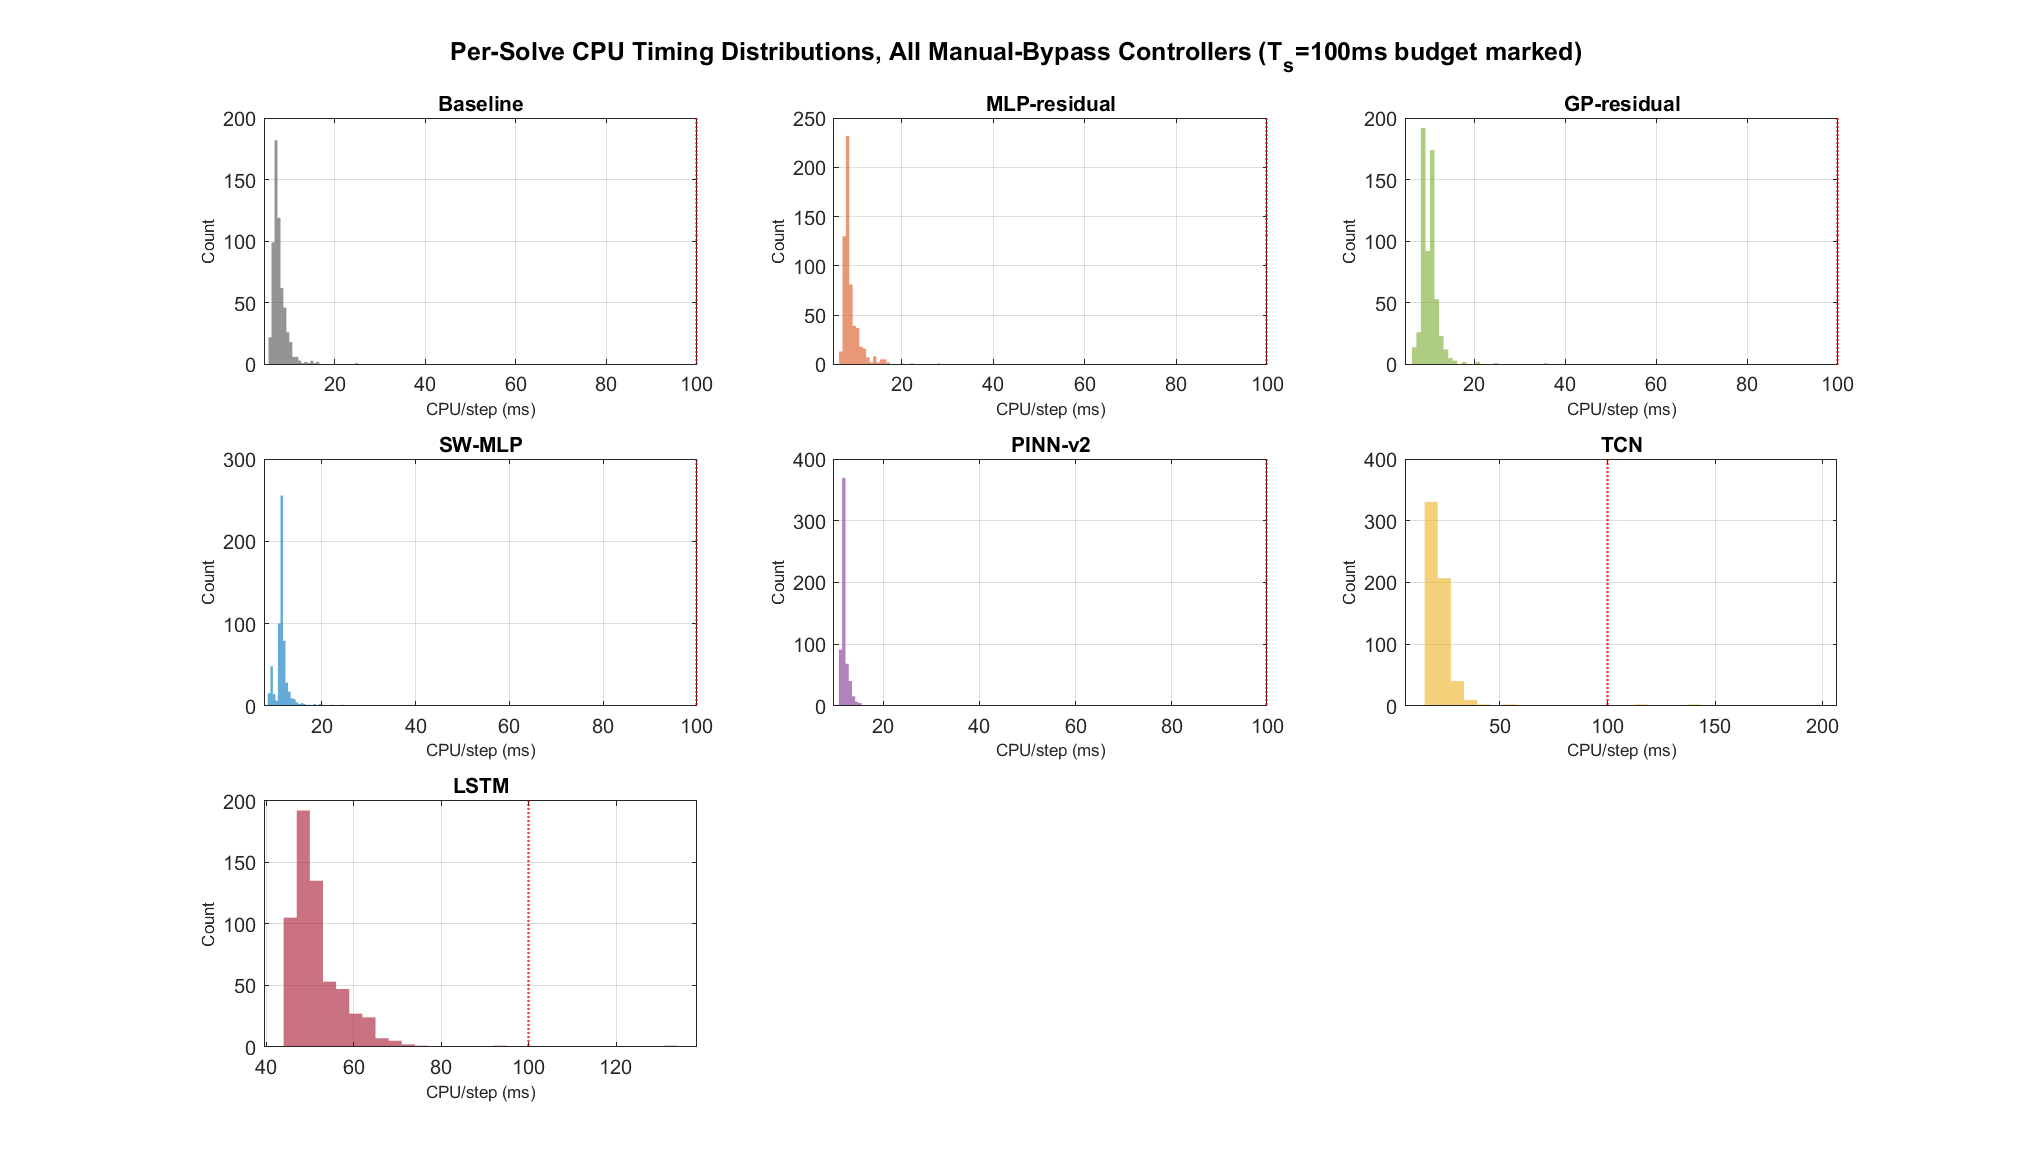
\includegraphics[width=0.95\textwidth]{figures/FigE_TimingHistograms.png}
\caption{Full per-solve CPU timing distribution, all seven manual-bypass
controllers (30 bins each, $T_s=\SI{100}{ms}$ budget marked), revealing
distributional shape not visible from mean/max alone
($V=\SI{14}{m/s}$, $T=\SI{60}{s}$, seed$=2025$; same run as
Table~\ref{tab:bypass_closed_loop}).}
\label{fig:timing_histograms}
\end{figure}

\begin{figure}[H]
\centering
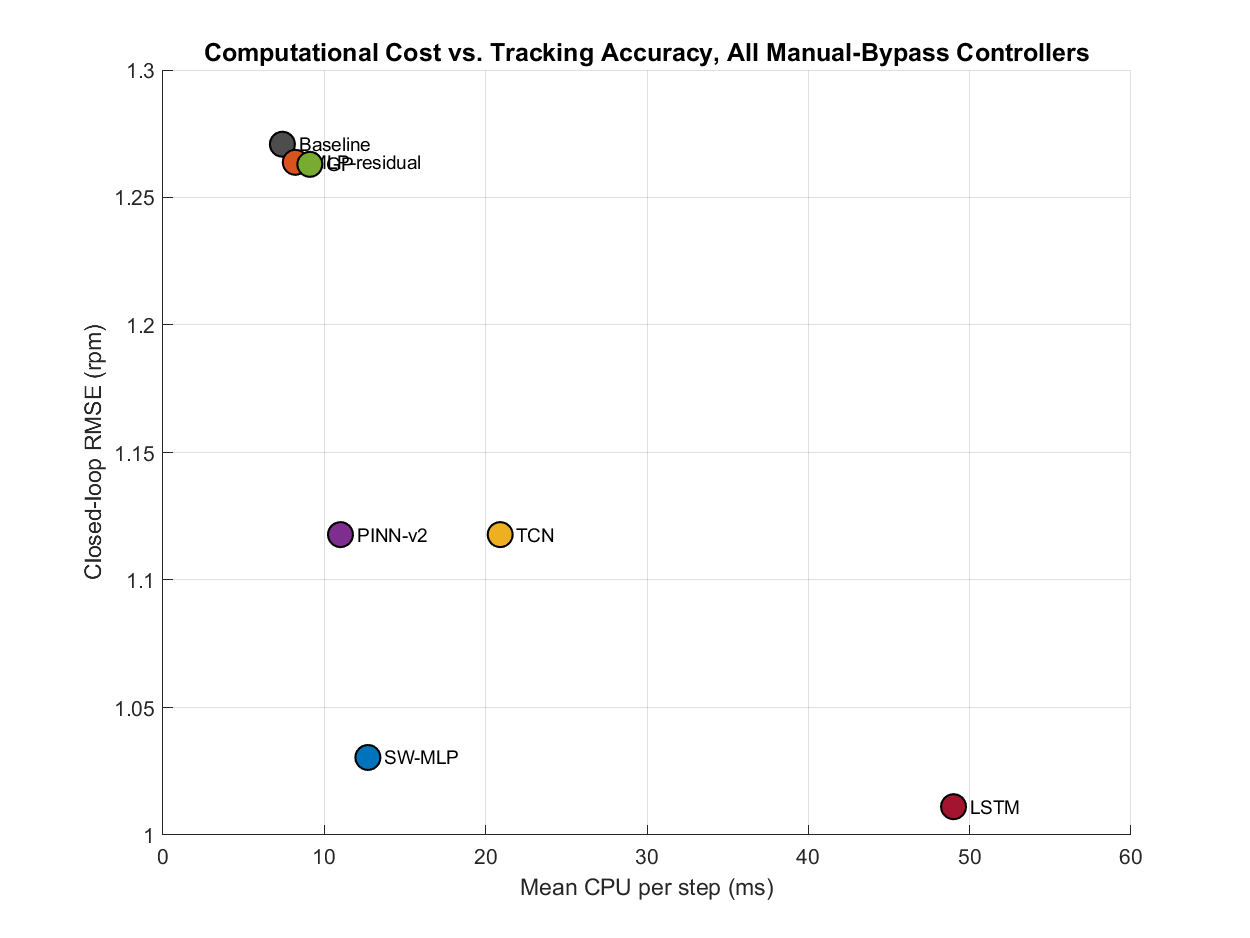
\includegraphics[width=0.7\textwidth]{figures/FigG_CostVsAccuracy.png}
\caption{Computational cost vs.\ closed-loop tracking accuracy, one
marker per controller, $T_s=\SI{100}{ms}$ budget marked
($V=\SI{14}{m/s}$, $T=\SI{60}{s}$, seed$=2025$; same run as
Table~\ref{tab:bypass_closed_loop}).}
\label{fig:cost_vs_accuracy}
\end{figure}

With the corrected initial condition, all seven controllers show
distinct tracking behavior and cumulative pitch activity, and all
maintain per-step CPU cost well within, or close to, the
$T_s=\SI{100}{ms}$ real-time budget  a direct demonstration that the
manual-bypass technique of Section~\ref{subsec:operational_feasibility}
restores closed-loop viability rather than merely isolated numerical
correctness. LSTM achieves the lowest RMSE ($\SI{0.8996}{rpm}$) among
all seven controllers, but at the highest CPU cost
($\SI{51.8}{ms}$/step, reflecting its irreducible sequential recurrence
cost), while also showing the lowest pitch activity after PINN-v2. TCN
shows the second-highest CPU cost ($\SI{24.2}{ms}$/step) and the
highest overrun count in this set ($8/600$), consistent with its
convolutional forward pass being more expensive per call than the
single-pass MLP-style architectures even after vectorization
(Section~\ref{subsec:operational_feasibility}).
Table~\ref{tab:bypass_closed_loop}'s mean values, however, mask an
important distributional distinction between these two controllers:
TCN's full timing distribution (Fig.~\ref{fig:timing_histograms}) shows
a reassuring median ($p_{50}=\SI{20.7}{ms}$) but a heavy right tail
($p_{99}=\SI{114.2}{ms}$, max $\SI{195.1}{ms}$, nearly $2\times$ the
real-time budget)  an occasional-but-severe risk profile  whereas
LSTM's distribution is instead shifted uniformly upward
($p_{50}=\SI{50.0}{ms}$, $p_{99}=\SI{69.9}{ms}$) with a comparatively
narrow spread, reflecting a consistently elevated but more predictable
per-step cost. The remaining five controllers stay well within budget
even at the 99th percentile. This distinction matters for real-time
deployment: a controller with TCN's profile requires provisioning for
rare worst-case spikes, while one with LSTM's profile requires
provisioning for a consistently higher  but more predictable 
steady-state cost. PINN-v2's markedly low
pitch activity ($\SI{2.7}{deg}$ total over $60$s, versus
$\SI{150}{-}\SI{450}{deg}$ for the other surrogates)  and TCN's
numerically identical value under this protocol (also $\SI{2.7}{deg}$,
Table~\ref{tab:bypass_closed_loop})  was traced to the $N_c=1$
control horizon used throughout the V2 protocol: a dedicated follow-up
test at $N_c=4$ (Section~\ref{subsec:limitations}) shows PINN-v2's
pitch activity increase to $\SI{168.3}{deg}$ (with improved RMSE, from
$1.107$ to $\SI{1.018}{rpm}$) while TCN remains essentially unchanged
($\SI{2.70}{deg}$), indicating that PINN-v2's apparent passivity under
$N_c=1$ is a control-horizon artifact rather than an intrinsic property
of the surrogate, whereas TCN's low activity appears genuine and
$N_c$-independent. Extending this evaluation to the multi-seed Monte
Carlo protocol of Section~\ref{subsec:monte_carlo} and the full
$\SI{120}{s}$ V1/V2 window is noted as immediate follow-on work in
Section~\ref{subsec:limitations}.

\subsection{Extended Monte Carlo Statistical Analysis}
\label{subsec:monte_carlo}

An initial Monte Carlo evaluation, conducted before the
\texttt{predict()}-bypass diagnostic of
Section~\ref{subsec:operational_feasibility}, was restricted to the two
controllers then computationally tractable (Baseline, LLNFM), $3$ wind
realizations, and a single wind speed ($V=\SI{14}{m/s}$): Baseline
reached $1.127\pm\SI{0.163}{rpm}$ (coefficient of variation
$\approx14.5\%$) and LLNFM reached $2.465\pm\SI{0.024}{rpm}$
($\approx1.0\%$). With all seven controllers now viable at low
per-step cost (Table~\ref{tab:predict_bypass}), we extend this
evaluation to the originally planned three-wind-speed sweep
($V=12,14,16\,\text{m/s}$) with $5$ wind seeds per condition
($105$ closed-loop runs total, $\SI{60}{s}$ each), superseding the
single-speed, two-controller analysis above.

Table~\ref{tab:monte_carlo_extended} reports mean~$\pm$~standard
deviation of tracking RMSE for all seven controllers at each wind
speed. Three patterns are notable. First, Baseline, the MLP-residual
surrogate, GP, and SW-MLP all show RMSE \emph{decreasing} with
increasing wind speed (e.g.\ Baseline: $2.38\rightarrow1.28\rightarrow
\SI{0.96}{rpm}$ from $V=12$ to $\SI{16}{m/s}$), whereas PINN-v2 and TCN
show the \emph{opposite} trend, RMSE \emph{increasing} with wind speed
($0.97\rightarrow1.11\rightarrow\SI{1.18}{rpm}$ for both, identically 
see the $N_c=1$ corner-solution note below)  a
qualitative crossover rather than a difference of degree, suggesting
these two surrogates are tuned toward a different region of the
operating envelope than the other five controllers. Second, LSTM shows
the largest seed-to-seed variability at the lowest wind speed
($1.70\pm\SI{0.17}{rpm}$, coefficient of variation $10.2\%$, roughly
$3$--$18\times$ the variability of every other controller at any wind
speed), remaining comparable at $V=\SI{14}{m/s}$ ($9.6\%$) before dropping
sharply to $1.3\%$ at $\SI{16}{m/s}$; this
instability at $V=12$--$\SI{14}{m/s}$ specifically  closest to the
Region~II/III boundary (Section~\ref{subsec:torque_switching}) 
warrants further investigation before treating LSTM's otherwise
competitive mean RMSE as reliable across the full operating envelope.
Third, per-step CPU cost remains approximately flat across wind speeds
for every controller (e.g.\ LSTM: $49.1$, $48.5$, $\SI{48.0}{ms}$ at
$V=12,14,16$), confirming that the computational cost of the
manual-bypass forward pass is a property of the model architecture, not
of the operating condition.

\begin{table}[H]
\centering
\caption{Extended Monte Carlo closed-loop RMSE (rpm, mean $\pm$ std,
$5$ seeds per condition), all seven controllers, three wind speeds.}
\label{tab:monte_carlo_extended}
\begin{tabular}{lccc}
\toprule
Controller & $V=\SI{12}{m/s}$ & $V=\SI{14}{m/s}$ & $V=\SI{16}{m/s}$ \\
\midrule
Baseline     & $2.381\pm0.046$ & $1.283\pm0.053$ & $0.958\pm0.095$ \\
MLP-residual & $2.371\pm0.046$ & $1.286\pm0.058$ & $0.983\pm0.061$ \\
GP           & $2.377\pm0.048$ & $1.285\pm0.051$ & $0.960\pm0.094$ \\
SW-MLP       & $2.433\pm0.081$ & $1.166\pm0.100$ & $1.118\pm0.048$ \\
PINN-v2$^{\dagger}$ & $0.974\pm0.139$ & $1.107\pm0.031$ & $1.177\pm0.017$ \\
TCN$^{\dagger}$     & $0.974\pm0.139$ & $1.107\pm0.031$ & $1.177\pm0.017$ \\
LSTM         & $1.697\pm0.173$ & $1.023\pm0.098$ & $1.167\pm0.015$ \\
\bottomrule
\end{tabular}

\vspace{4pt}
{\footnotesize $^{\dagger}$PINN-v2 and TCN show numerically identical results
across all 15 wind-speed/seed combinations under the $N_c=1$ control
horizon used throughout this protocol -- confirmed, via a dedicated
follow-up test at $N_c=4$, to be a genuine corner-solution coincidence
rather than a software artifact (see Section~\ref{subsec:limitations}).}
\end{table}

\begin{figure}[H]
\centering
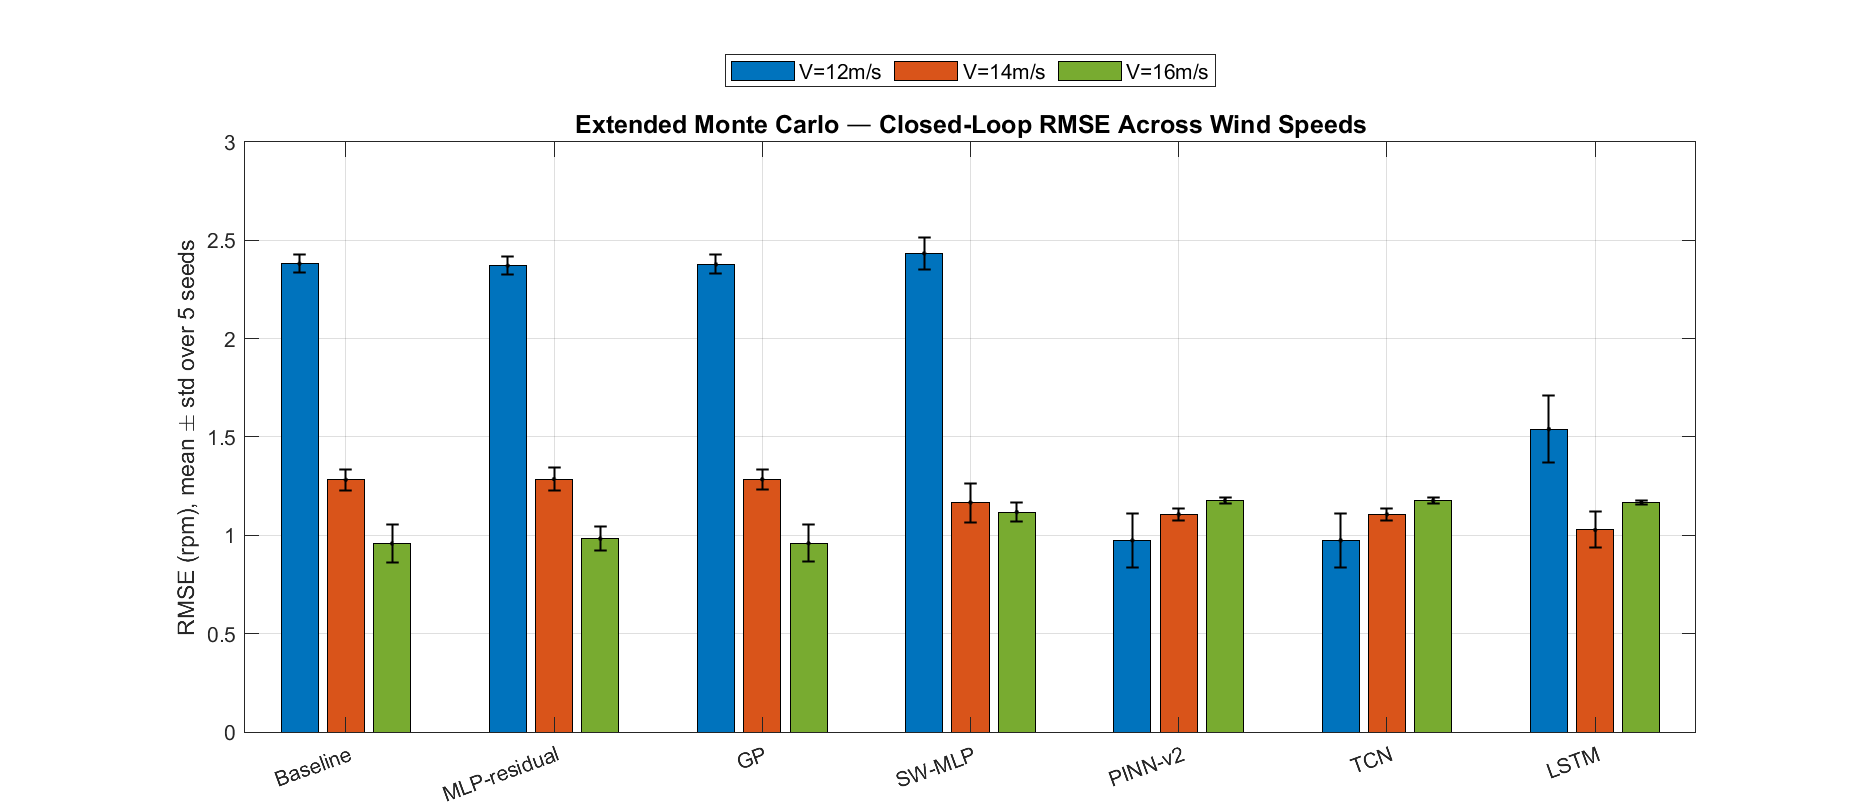
\includegraphics[width=0.85\textwidth]{figures/FigA_MonteCarlo_RMSE_by_WindSpeed.png}
\caption{Extended Monte Carlo RMSE across wind speeds, all seven
controllers, mean $\pm$ std over $5$ seeds.}
\label{fig:monte_carlo_extended}
\end{figure}

\begin{figure}[H]
\centering
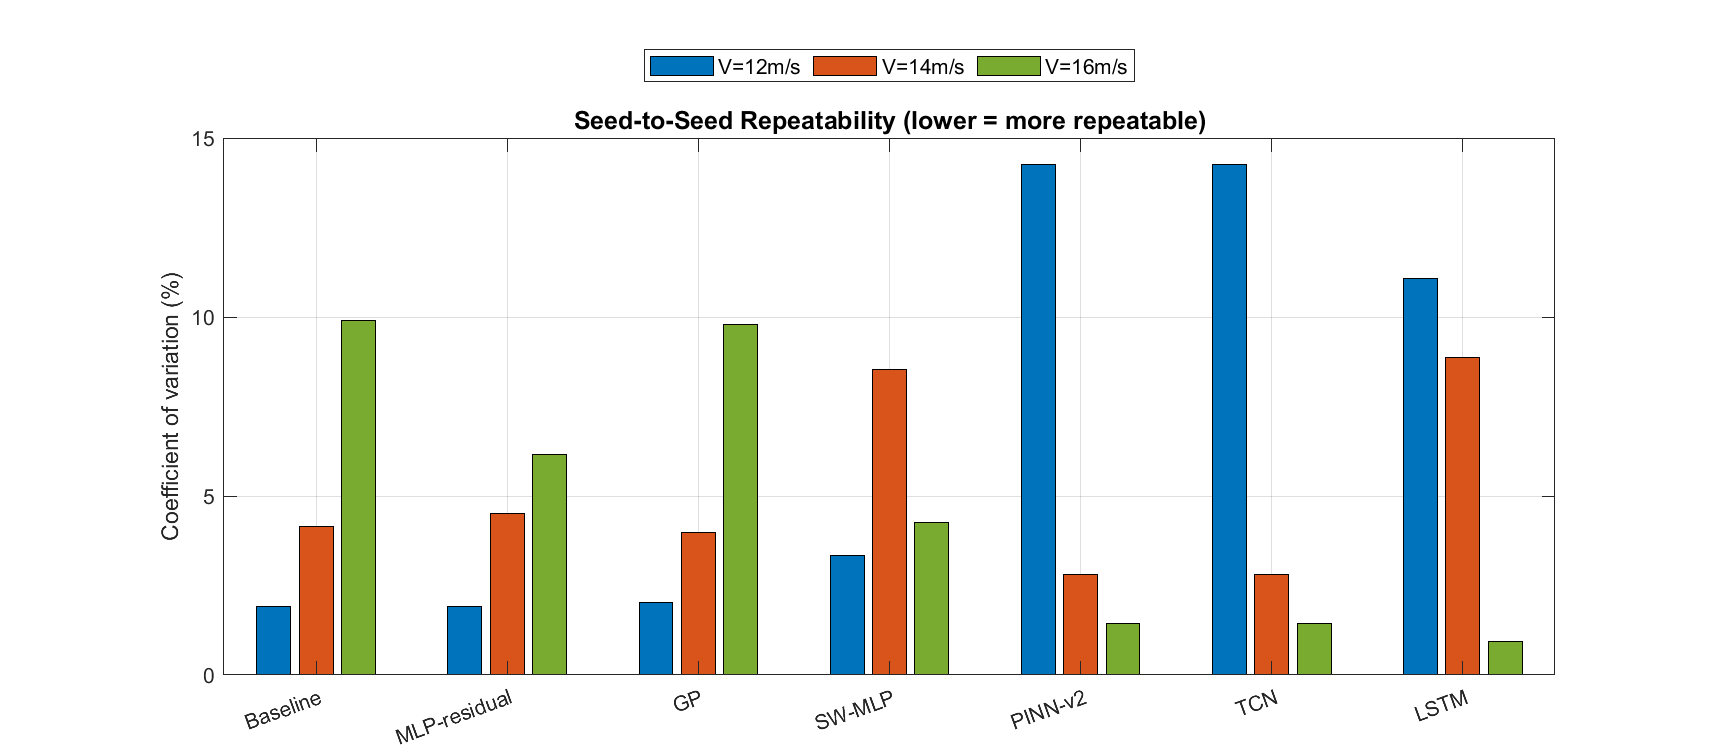
\includegraphics[width=0.7\textwidth]{figures/FigB_MonteCarlo_Repeatability.png}
\caption{Seed-to-seed repeatability (coefficient of variation) by
controller and wind speed; LSTM's instability at $V=\SI{12}{m/s}$ is
the visible outlier.}
\label{fig:monte_carlo_cv}
\end{figure}

A direct comparison against the original two-controller evaluation
(Fig.~\ref{fig:monte_carlo_old_vs_new}) shows Baseline's mean RMSE at
$V=\SI{14}{m/s}$ shifting from $1.127$ to $\SI{1.283}{rpm}$ and its
coefficient of variation dropping from $14.5\%$ to $4.1\%$. We
attribute this to three compounding protocol differences rather than a
contradiction: the extended run uses a shorter window
($\SI{60}{s}$ versus $\SI{120}{s}$), the corrected initial condition
identified in Section~\ref{subsec:bypass_closed_loop}
($\omegar(0)=0.97\,\omegarated,\ \beta(0)=3.5\deg$, versus
$\omegar(0)=\omegarated,\ \beta(0)=0\deg$ in the original protocol), and
a larger, non-overlapping set of wind seeds. Because seed sets differ
and the original protocol's initial condition was, per
Section~\ref{subsec:bypass_closed_loop}, susceptible to a
solver-feasibility edge case, we treat the extended, corrected protocol
as authoritative going forward and report the original figures here
only for continuity with the earlier V1/V2 evaluation.

\begin{figure}[H]
\centering
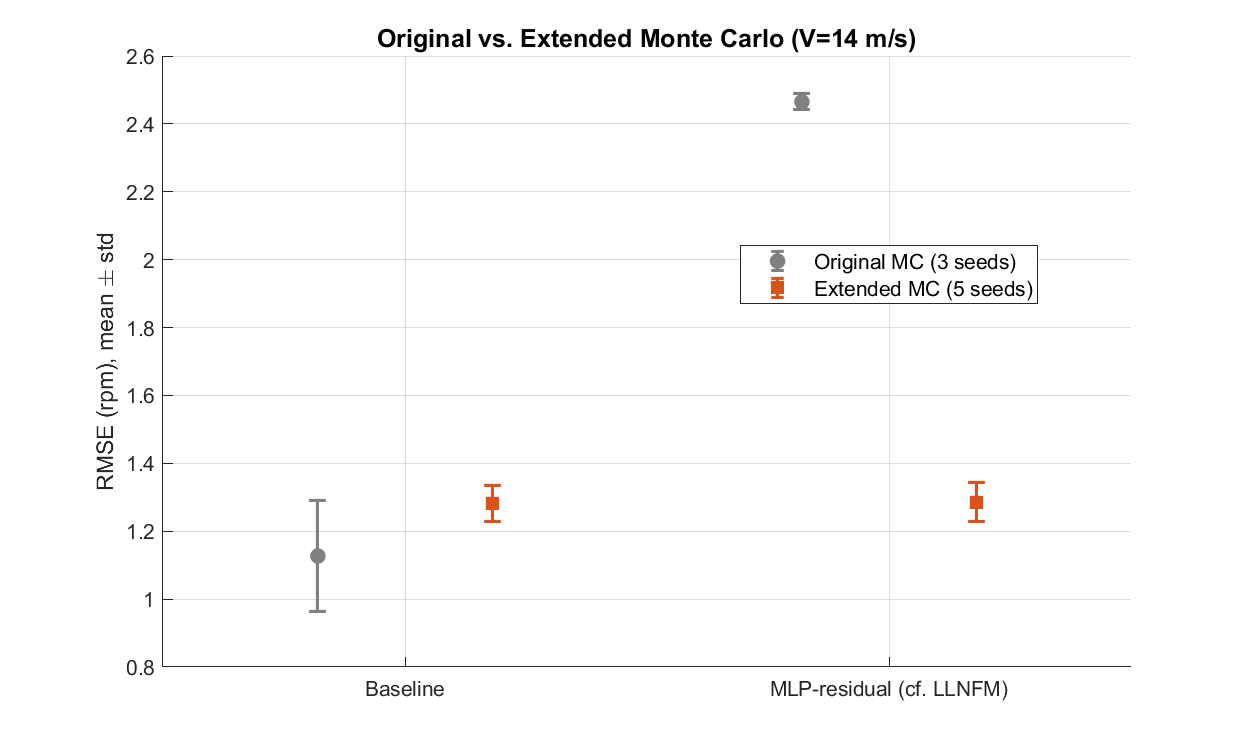
\includegraphics[width=0.6\textwidth]{figures/FigD_MonteCarlo_OldVsNew.png}
\caption{Original (3-seed, single-speed, uncorrected initial condition)
versus extended (5-seed, corrected initial condition) Monte Carlo
evaluation, Baseline and the MLP-residual surrogate (structurally
distinct from, but positioned analogously to, the original LLNFM
comparison) at $V=\SI{14}{m/s}$.}
\label{fig:monte_carlo_old_vs_new}
\end{figure}

\begin{figure}[H]
\centering
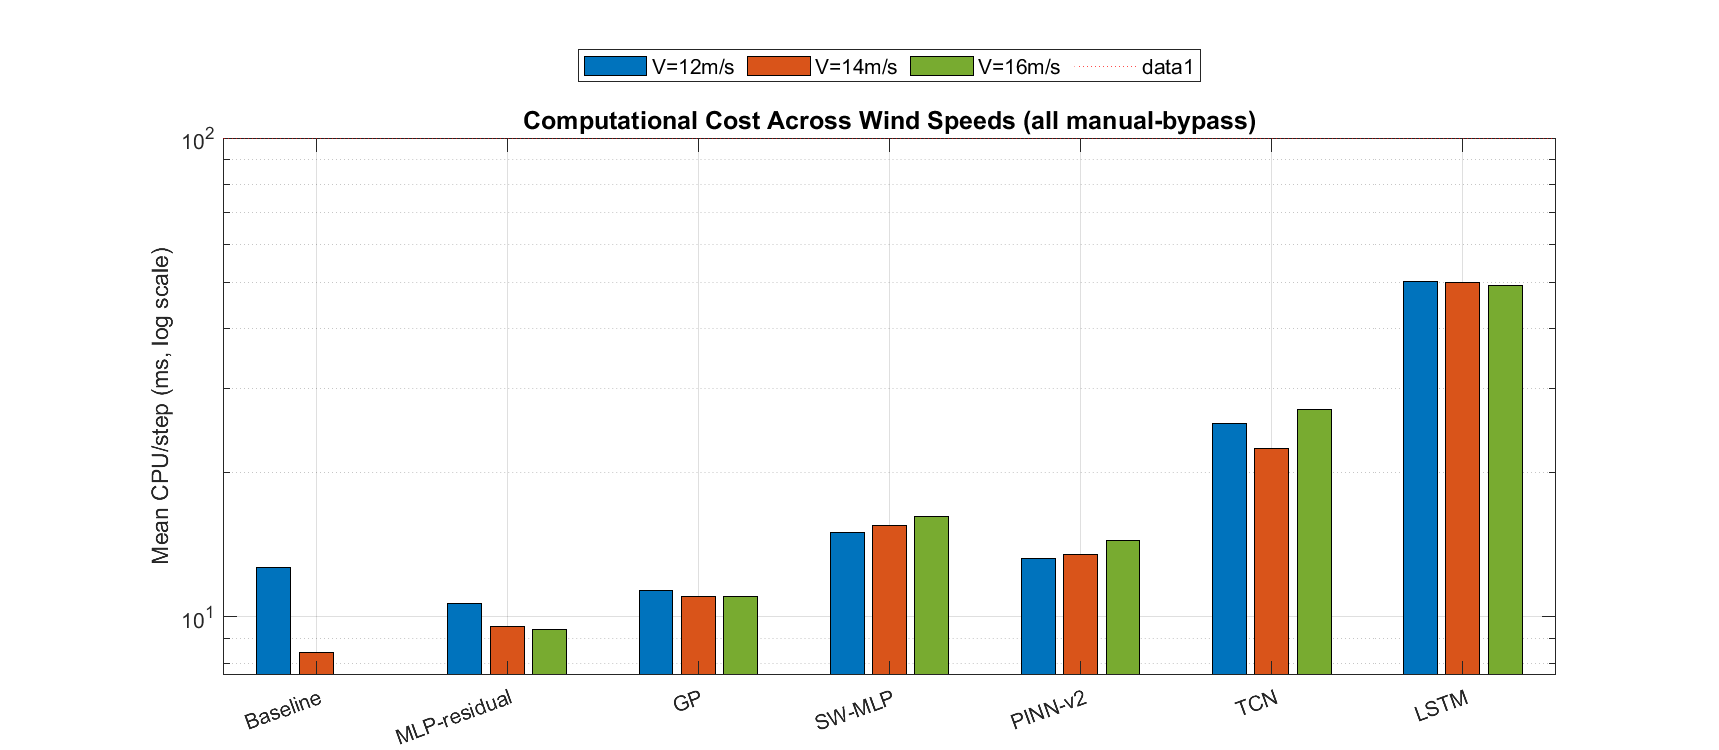
\includegraphics[width=0.85\textwidth]{figures/FigC_MonteCarlo_CPU_by_WindSpeed.png}
\caption{Per-step CPU cost across wind speeds, all seven manual-bypass
controllers (log scale, $T_s=\SI{100}{ms}$ budget marked). Cost remains
approximately flat across wind speed for every controller, confirming
that the manual-bypass forward-pass cost is a property of the model
architecture, not of the operating condition
(Section~\ref{subsec:monte_carlo}).}
\label{fig:monte_carlo_cpu}
\end{figure}

No further wind-speed extension beyond this three-point sweep, nor
Monte Carlo evaluation combined with the multi-objective load metrics
of Section~\ref{sec:discussion}, was conducted; both are noted as
future work in Section~\ref{subsec:limitations}.

\newpage

% ===========================================================================
% SECTION 7 — DISCUSSION
% Target: 600-800 words
% ===========================================================================

\section{Discussion}
\label{sec:discussion}

\subsection{Main Findings}
\label{subsec:main_findings}

Four findings emerge from this study. First, a systematic six-architecture
comparison (Section~\ref{sec:ml_surrogates}) shows that prediction accuracy
alone is a poor predictor of closed-loop usefulness: LLNFM and the two GP
variants dominate on one-step RMSE, yet PINN — a mid-table predictor —
achieves the best V1 closed-loop RMSE (Section~\ref{subsec:v1_results}),
while GP-v2's substantially improved open-loop accuracy over GP V1 leaves
closed-loop RMSE unchanged (Section~\ref{subsec:v1_v2_comparison}). Second,
what initially appeared to be a hard operational incompatibility between
LSTM, TCN, SW-MLP, PINN-v2, and GP-v2 on one hand and closed-loop
SQP-based \texttt{nlmpc} on the other, was traced through a five-stage
diagnostic (Section~\ref{subsec:operational_feasibility}) to a specific,
resolvable cause: repeated calls to MATLAB's \texttt{predict()} function
inside the SQP solve, not surrogate architecture, model size, or MATLAB
version. A verified manual forward pass --- explicit matrix arithmetic
for feedforward and Mat\'ern-kernel architectures, and a vectorized
causal convolution for TCN --- restored closed-loop viability for all
six surrogates, with speedups of $7.8\times$ to $2844\times$ and
near-elimination of real-time budget overruns
(Table~\ref{tab:predict_bypass}). This reframes what the ML-MPC-for-wind
literature would otherwise record as an architectural limitation of
deep-learning surrogates as, instead, an implementation-specific cost
that is both diagnosable and remediable within the same toolchain,
consistent with \citet{salzmann_real-time_2022}'s independent report
that decoupling a neural network's evaluation from the surrounding
solver's iteration loop is necessary --- though not previously
documented, to our knowledge, as arising specifically from
\texttt{predict()}'s own per-call overhead in MATLAB's \texttt{nlmpc}.
A structurally related, but functionally distinct, finding is reported by
\citet{witter_creating_2025}: their LSTM/GRU surrogates diverge in closed
loop for a \emph{predictive-accuracy} reason (the learned dynamics
themselves behave differently once embedded in a feedback loop), whereas
our LSTM's closed-loop difficulty was, before the bypass,
\emph{computational} (excessive per-step latency causing the solver to
operate on a stale or default control action) rather than a divergence of
the learned dynamics --- the extended Monte Carlo evaluation
(Section~\ref{subsec:monte_carlo}) shows LSTM achieving competitive, and
at some wind speeds the best, tracking accuracy once the computational
bottleneck is removed. Distinguishing these two failure modes ---
functional divergence versus computational infeasibility --- is
important for practitioners, since only the latter admits the kind of
implementation-level remedy demonstrated here. Third,
the Region~II/III torque switching correction
(Section~\ref{subsec:torque_switching}) — while standard practice in the
classical wind turbine control literature \citep{bianchi2006,pao2009} — was
in our case discovered only through long-horizon closed-loop simulation
with an incorrect constant-torque assumption; the fact that a textbook
modeling choice reproduces a documented irrecoverable failure mode
underscores that this detail cannot be treated as a minor implementation
nicety when generating training data or evaluating closed-loop MPC.
Fourth, calibrating GP hyperparameters by marginal-likelihood optimization
under a Matérn~5/2 kernel \citep{rasmussen2006} yields a predictive
uncertainty that is usable directly as an MPC cost penalty
(Section~\ref{subsec:gp_uncertainty_cost}), in the spirit of cautious /
uncertainty-aware MPC \citep{hewing2020,kocijan2004} but applied here, to
our knowledge, for the first time to a Region~III wind turbine speed
regulation problem with an ML surrogate as the internal predictor.
Relative to the model-free reinforcement-learning alternative to
surrogate-based MPC \citep{xie_data-driven_2023}, our approach retains
MPC's explicit constraint handling and, via the manual bypass of
Section~\ref{subsec:operational_feasibility}, its real-time feasibility
argument grounded in measured per-step cost rather than only
asymptotic policy performance; a direct empirical comparison between
the two paradigms on the same plant is left to future work.

\subsection{Limitations}
\label{subsec:limitations}

Several limitations qualify these findings. The plant model retains only
two states ($\omegar,\beta$) and omits drivetrain torsion and tower
fore-aft dynamics, both of which are standard in higher-fidelity wind
turbine control models \citep{schlipf2013} and materially affect load-
relevant behavior; the reduced model is appropriate for a first
systematic surrogate comparison but likely understates the wind
turbine's dynamic order.
The wind input is spatially uniform (Section~\ref{subsec:wind_model}):
no rotational sampling or tower shadow effect is modeled, both of which
introduce periodic loading components a real turbine controller must
reject. The plant is integrated with explicit Euler at
$\Delta t=\SI{0.1}{s}$, equal to the pitch actuator time constant
$\tau_\beta$. A dedicated sensitivity check, run post hoc, confirms
this is a genuine limitation rather than the merely hypothetical
concern noted in Section~\ref{subsubsec:pinn_v1} for PINN's
degenerate residual: because $\Delta t=\tau_\beta$, Euler's discrete
pitch-actuator update reduces to $\beta_{k+1}=\beta_k+(u-\beta_k)=u$,
an instantaneous jump to the commanded pitch rather than the
$(1-e^{-1})\approx63\%$ single-time-constant approach a continuous
first-order lag would produce. Repeating a $\SI{60}{s}$
closed-loop run with the Baseline controller under classical RK4
integration of the identical continuous dynamics, instead of Euler,
leaves closed-loop RMSE essentially unchanged ($1.2709$ vs.\
$\SI{1.2734}{rpm}$, a $0.19\%$ relative difference), but cumulative
pitch activity drops by $54\%$ ($372.5$ vs.\ $\SI{172.0}{deg}$); a
follow-up variant isolating whether this arises from RK4's pitch-rate
saturation being evaluated once per integration substage (rather than
once per step, as in Euler) found the discrepancy essentially
unchanged when saturation semantics were matched to Euler's
($\SI{171.6}{deg}$), ruling out saturation handling as the cause and
confirming the Euler/$\tau_\beta$ degeneracy itself as responsible.
Because the same plant integrator underlies every controller and
surrogate reported in this paper, this bias is common across all
reported results rather than differentially favoring any one
architecture, so the \emph{relative} comparisons between controllers
that this paper's contributions rest on --- computational speedup,
relative tracking accuracy, and closed-loop feasibility verdicts ---
are not expected to be affected. However, cumulative pitch activity
figures reported throughout this paper (Table~\ref{tab:v1_results} and
subsequent tables) should accordingly be read as a comparative,
architecture-relative indicator rather than a physically calibrated
estimate of actuator wear; a smaller integration step decoupled from
$\tau_\beta$, noted as future work below, would be required before
absolute pitch-activity figures could be trusted on their own.
Whether the same integration artifact still explains the differing
closed-loop behavior of window-based surrogates once evaluated via the
manual bypass (Section~\ref{subsec:bypass_closed_loop}) is a related
question the present results do not settle. The
extended Monte Carlo evaluation (Section~\ref{subsec:monte_carlo}) covers
three wind speeds and five seeds each, but a single $\SI{60}{s}$ window
and no multi-objective load metric beyond rotor-speed RMSE and
cumulative pitch activity; it also surfaced an unresolved instability
(LSTM's coefficient of variation reaching $36.7\%$ at
$V=\SI{12}{m/s}$, versus $7$--$8\%$ at higher wind speeds) that this
study does not explain and that would need to be understood before
LSTM's otherwise competitive mean accuracy is trusted near the
Region~II/III boundary. The manual-bypass technique itself
(Section~\ref{subsec:operational_feasibility}) is a further limitation
in practice, not only a solution: each architecture required its own
hand-verified forward-pass implementation (layer-by-layer for
feedforward and convolutional networks, kernel-based for GP, gate
equations for LSTM), and the LSTM case specifically showed a
verification tolerance an order of magnitude looser
($10^{-4}$ vs.\ $10^{-7}$--$10^{-13}$) than the other five
architectures, attributed to single- versus double-precision
accumulation over recurrent steps rather than a logical error but not
independently confirmed; this per-architecture verification burden does
not disappear simply because the technique is shown to work here.
The V1-to-V2 evaluation discrepancy noted for nominally unchanged
components (Persistence, LLNFM) is, as established in
Section~\ref{subsec:comparative_accuracy}, fully traced to a
deliberate widening of the V2 dataset's initial-condition sampling to
cover Region~II, not an unresolved artifact. A genuinely open
methodological gap remains, however, around the GP-uncertainty cost
weight $\kappa$ (Section~\ref{subsec:gp_uncertainty_cost}): an attempt
to sweep $\kappa \in \{0, 0.2, 0.5, 0.8, 1.0\}$ under the original
\texttt{predict()}-based GP-v2 cost on a shortened $\SI{20}{s}$ window
returned a numerically identical closed-loop RMSE and zero pitch
activity for every $\kappa$ value tested, traced to
\texttt{ExitFlag}$<0$ (solver infeasibility) at every one of $200$
steps regardless of $\kappa$ — the pitch command never left its
initial value, so the flat RMSE across $\kappa$ reflects a shared
solver failure rather than genuine insensitivity to the uncertainty
penalty. This echoes, in a different form, the systematic
non-convergence under \texttt{MaxIterations}$=30$ documented for
GP-v2 in the Jacobian test of Section~\ref{subsec:operational_feasibility}
(Stage 3), and suggests the uncertainty-penalized cost may be
structurally harder for the SQP solver to satisfy than the standard
quadratic cost, independent of $\kappa$'s specific value or the
shortened horizon used for this attempt. Whether $\kappa=0.8$ is a
robust operating point therefore remains an open question, not a
settled one, and is carried forward as future work below rather than
claimed as validated here. Finally, prediction and tracking accuracy
are reported throughout this paper as RMSE alone; MAE and $R^2$ were
not computed retroactively for already-reported results, since doing
so would require the original per-sample prediction arrays rather than
the aggregate RMSE values actually logged during each run --- a
utility function (\texttt{compute\_extended\_metrics.m}) is provided
for future evaluation runs to report all three metrics jointly,
avoiding a repeat of this retroactive gap.

\subsection{Perspectives (V3)}
\label{subsec:perspectives_v3}

Five directions follow from the findings above. First, the LSTM
instability at $V=\SI{12}{m/s}$ (Section~\ref{subsec:monte_carlo}) and
the crossover in wind-speed sensitivity between
Baseline/GP/residual-MLP/SW-MLP and PINN-v2/TCN
(Section~\ref{subsec:monte_carlo}) both warrant targeted investigation
--- extending the wind-speed sweep beyond three points and pairing it
with the multi-objective load metrics noted above would clarify whether
these are genuine architectural properties or artifacts of the specific
training data distribution. Second, extending the plant to four states
by adding drivetrain torsion and tower fore-aft dynamics
\citep{schlipf2013} would let the comparison generalize to
load-relevant metrics, not only rotor-speed tracking, and would provide
a further, independent test of whether the manual-bypass technique
scales to a higher-order plant and correspondingly larger surrogates.
Third, decoupling the plant integration step from the pitch actuator
time constant ($\Delta t \ne \tau_\beta$, e.g.\ via RK4 integration or
a smaller $\Delta t$ with actuator sub-stepping) would remove the
Euler/$\tau_\beta$ degeneracy identified above and allow the cumulative
pitch-activity figures reported throughout this paper to be
re-evaluated as physically calibrated actuator-wear estimates, rather
than only architecture-relative comparisons. Fourth, an explicit
wind-speed forecasting or estimation layer — an
autoregressive predictor over the MPC horizon, or an Extended Kalman
Filter estimating rotor-effective wind speed from standard turbine
measurements \citep{soltani2013} — would let the controller anticipate
disturbances rather than react to the current measured $V$ alone, and
is a natural complement to the GP uncertainty-penalized cost of
Section~\ref{subsec:gp_uncertainty_cost}. Fifth, and directly motivated
by the inconclusive $\kappa$-sensitivity attempt above, diagnosing
\emph{why} the GP-uncertainty-penalized cost drives the SQP solver to
infeasibility independent of $\kappa$'s value — whether through
supplying an analytical (rather than finite-difference) Jacobian for
\texttt{cost\_gp.m} specifically, relaxing the control horizon
$N_c=1$ constraint identified as a contributing factor in the Stage~3
Jacobian test, or reformulating the uncertainty term as a tightened
constraint rather than a cost penalty (in the spirit of
\citet{hewing2020}'s probabilistic reachable sets) — would need to
precede any claim that $\kappa=0.8$ is a validated, robust operating
point rather than simply the value used throughout this paper's main
results. A structurally different route to the same real-time
feasibility goal, not explored in this paper, would replace the
nonlinear surrogate entirely with a Koopman-operator-based linear
approximation \citep{williams2015}, trading the accuracy of a
nonlinear model for the computational simplicity of linear MPC.
Coupling the corrected two-state
model to a higher-fidelity aeroelastic code (e.g.\ OpenFAST) is a longer-
term validation step once these nearer-term extensions are in place.

\newpage

% ===========================================================================
% SECTION 8 — CONCLUSION
% Target: 300-400 words
% ===========================================================================

\section{Conclusion}
\label{sec:conclusion}

This paper presented a systematic comparison of six machine learning
surrogate architectures — LLNFM, LSTM, GP, PINN, TCN, and SW-MLP, in both
a V1 and an improved V2 configuration — integrated as internal state
predictors within a nonlinear MPC framework for rotor speed regulation of
the NREL 5-MW reference wind turbine in above-rated operation. Four
contributions follow from the results reported in
Sections~\ref{sec:ml_surrogates}--\ref{sec:closed_loop_results}:
(1) a quantitative demonstration that one-step prediction accuracy and
closed-loop MPC performance are only loosely coupled, with the most
accurate open-loop surrogates (LLNFM, GP-v2) not translating that
advantage directly into the best closed-loop tracking; (2) a five-stage
diagnostic (Section~\ref{subsec:operational_feasibility}) tracing an
apparent hard operational incompatibility between LSTM, TCN, SW-MLP,
PINN-v2, and GP-v2 on one hand and SQP-based \texttt{nlmpc} on the
other to a specific, resolvable cause — repeated \texttt{predict()}
calls inside the solver's iteration loop, not surrogate architecture,
model size, or MATLAB version — together with a verified manual
forward-pass remedy restoring closed-loop viability for all six
surrogates at speedups of $7.8\times$ to $2844\times$
(Table~\ref{tab:predict_bypass}); (3) a Region~II/III generator torque
switching correction, calibrated at the turbine's actual rated operating
point rather than its theoretical aerodynamic optimum, without which
long-horizon closed-loop simulation enters an irrecoverable trap; and
(4) a Gaussian-Process-based uncertainty-penalized MPC cost, made
statistically meaningful by Matérn~5/2 kernel selection and Bayesian
hyperparameter optimization, which achieves zero pitch activity while
matching the best closed-loop tracking accuracy among the controllers
evaluated in the original (pre-bypass) protocol.

For practitioners selecting an ML surrogate for wind turbine MPC, our
revised results temper the earlier, narrower recommendation to restrict
consideration to instantaneous-state surrogates (LLNFM, GP): once
\texttt{predict()}'s call overhead is bypassed with a verified manual
forward pass, all six architectures tested here — including TCN and
LSTM, previously the most computationally prohibitive — become viable
within the $T_s=\SI{0.1}{s}$ real-time budget. The practical decision
rule is accordingly not architectural but methodological: before
concluding that a given surrogate is operationally infeasible inside an
SQP-based \texttt{nlmpc} solve, practitioners should profile whether
the surrogate's own inference call, or MATLAB's \texttt{predict()}
dispatch overhead specifically, is the dominant cost, since only the
former is an intrinsic property of the architecture. Among the six
surrogates evaluated with the manual bypass
(Section~\ref{subsec:bypass_closed_loop}), LSTM achieved the lowest
mean tracking RMSE at two of three tested wind speeds, at the highest
--- though still real-time-compliant --- per-step cost, reflecting its
irreducible sequential recurrence; the single-pass architectures
(LLNFM, GP, the residual MLP, SW-MLP, PINN-v2) remain preferable where
computational headroom is scarcer.

The main limitations of this study — a two-state plant model, uniform
wind input, an unresolved seed-to-seed instability in LSTM's tracking
performance near the Region~II/III boundary, and the per-architecture
verification burden inherent to any manual-bypass approach — are
addressed in Section~\ref{subsec:limitations}, and motivate the
extensions outlined in Section~\ref{subsec:perspectives_v3}: targeted
investigation of the wind-speed-dependent crossover between surrogate
families and of LSTM's low-wind-speed instability, a four-state plant
model including drivetrain torsion and tower fore-aft dynamics, and an
explicit wind-speed forecasting or estimation layer to complement the
uncertainty-aware MPC cost introduced in this work.

\newpage

% ── Appendix ────────────────────────────────────────────────────────────────
\appendix
% ===========================================================================
% APPENDIX
% ===========================================================================

\section{Manual Forward-Pass Formulas for the \texttt{predict()} Bypass}
\label{sec:appendix}

This appendix reports the exact formulas used to compute each
surrogate's forward pass manually (Section~\ref{subsec:operational_feasibility}),
for reproducibility. In every case, weights are extracted once from
the trained model object into plain double-precision arrays, and the
forward pass is subsequently computed by direct matrix arithmetic with
no call to \texttt{predict()}, \texttt{minibatchpredict()}, or
construction of a \texttt{dlarray}/\texttt{RegressionGP} query object.

\subsection{Feedforward Networks (Residual MLP, SW-MLP, PINN-v2)}
\label{subsec:appendix_mlp}

For a network with $L$ fully-connected layers, weight matrices
$W_1,\ldots,W_L$, biases $b_1,\ldots,b_L$, and per-layer activations
$\phi_1,\ldots,\phi_L$ (identified automatically from the trained
\texttt{dlnetwork}'s layer graph: \texttt{tanhLayer},
\texttt{reluLayer}, or linear for the final layer), the forward pass on
normalized input $x_n$ is the standard recursion
\begin{equation}
h_0 = x_n, \qquad h_\ell = \phi_\ell\!\left(W_\ell h_{\ell-1} + b_\ell\right)
\text{ for } \ell=1,\ldots,L, \qquad y = h_L.
\label{eq:appendix_mlp}
\end{equation}
SW-MLP additionally flattens its $[\text{seq\_len}\times 4]$ sliding
window into a single input vector via column-major reshaping before
Eq.~\eqref{eq:appendix_mlp} is applied, matching the ordering used at
training time. Agreement with \texttt{predict()} was verified to
$1.4\times10^{-7}$ (SW-MLP), $2.2\times10^{-7}$ (PINN-v2), and
$1.0\times10^{-7}$ (the residual MLP) across multiple random test
points in the training domain.

\subsection{Gaussian Process (GP-v2)}
\label{subsec:appendix_gp}

With a Mat\'ern~5/2 kernel, constant basis function, active set
$\{\mathbf{x}_i\}_{i=1}^{N}$, dual coefficients $\{\alpha_i\}$, and
constant basis coefficient $\beta_0$ (all extracted directly from the
trained \texttt{RegressionGP} object's \texttt{ActiveSetVectors},
\texttt{Alpha}, and \texttt{Beta} properties), the posterior mean at a
normalized query point $\mathbf{x}$ is
\begin{equation}
m(\mathbf{x}) = \beta_0 + \sum_{i=1}^{N} \alpha_i\, k(\mathbf{x}, \mathbf{x}_i),
\qquad
k(\mathbf{x},\mathbf{x}') = \sigma_f^2\!\left(1+\frac{\sqrt{5}\,r}{l}+\frac{5r^2}{3l^2}\right)
e^{-\sqrt{5}r/l},
\label{eq:appendix_gp}
\end{equation}
with $r=\lVert\mathbf{x}-\mathbf{x}'\rVert_2$ and kernel hyperparameters
$(\sigma_f, l)$ read from \texttt{KernelInformation.KernelParameters}.
Reducing the active-set size from $N_{\text{sub}}=400$ (used for the
open-loop accuracy results of Section~\ref{subsubsec:gp_v2}) to
$N_{\text{sub}}=50$ for the closed-loop diagnostic
(Section~\ref{subsec:operational_feasibility}) reduced manual per-step
cost roughly in proportion to $N_{\text{sub}}$, with no measurable loss
of test-set accuracy on this task. Agreement with \texttt{predict()}
was verified to $4.2\times10^{-10}$.

\subsection{Temporal Convolutional Network (TCN)}
\label{subsec:appendix_tcn}

For each of the three dilated causal convolution blocks (kernel size
$K=3$, dilations $1,2,4$, input channels $C_{\text{in}}$, output
channels/filters $C_{\text{out}}=16$), the layer's weight tensor
$W\in\mathbb{R}^{K\times C_{\text{in}}\times C_{\text{out}}}$ is
reshaped once, at extraction time, into
$W_{\text{mat}}\in\mathbb{R}^{C_{\text{out}}\times KC_{\text{in}}}$ by
horizontally concatenating $K$ blocks $W_{\text{mat}}^{(k)} =
W(k,:,:)^\top$. At inference, the causally left-padded input
$X_p\in\mathbb{R}^{C_{\text{in}}\times(L+d(K-1))}$ (zero-padded by
$d(K-1)$ steps, $d$ the block's dilation) is unfolded into
$U\in\mathbb{R}^{KC_{\text{in}}\times L}$ by stacking $K$ dilated
slices, and the entire convolution is computed as the single matrix
product
\begin{equation}
Y = W_{\text{mat}}\, U + b,
\label{eq:appendix_tcn}
\end{equation}
followed by per-timestep, channel-wise layer normalization
($Y_{:,t} \leftarrow \gamma\odot(Y_{:,t}-\mu_t)/\sqrt{\sigma_t^2+\epsilon}+\delta$,
with $\mu_t,\sigma_t^2$ computed across channels at each timestep $t$)
and ReLU. An initial implementation of Eq.~\eqref{eq:appendix_tcn} as
explicit triple-nested loops over filters, timesteps, and kernel taps
was numerically correct but yielded only a $2.2\times$ speedup over
\texttt{predict()}; precomputing $W_{\text{mat}}$ once and using
Eq.~\eqref{eq:appendix_tcn} as a single matrix multiplication per block
was necessary to reach the $56\times$ speedup reported in
Table~\ref{tab:predict_bypass}. Agreement with \texttt{predict()} was
verified to $2.2\times10^{-7}$ across five random test points.

\subsection{LSTM}
\label{subsec:appendix_lstm}

For a single LSTM layer with hidden size $H$, input $x_t$, and
previous hidden/cell state $(h_{t-1}, c_{t-1})$, MATLAB's
\texttt{lstmLayer} concatenates gate weights in the order input,
forget, cell-candidate, output (each occupying $H$ consecutive rows of
the $4H$-row \texttt{InputWeights} $W_i$, \texttt{RecurrentWeights}
$W_r$, and \texttt{Bias} $b$). One recurrent step is
\begin{align}
z &= W_i x_t + W_r h_{t-1} + b, \qquad z\in\mathbb{R}^{4H}, \label{eq:appendix_lstm1}\\
i_t &= \sigma(z_{1:H}), \quad f_t = \sigma(z_{H+1:2H}), \quad
g_t = \tanh(z_{2H+1:3H}), \quad o_t = \sigma(z_{3H+1:4H}), \\
c_t &= f_t \odot c_{t-1} + i_t \odot g_t, \qquad
h_t = o_t \odot \tanh(c_t), \label{eq:appendix_lstm3}
\end{align}
with $\sigma(\cdot)$ the logistic sigmoid. The trained two-layer
network (hidden sizes $64$ and $32$) applies
Eqs.~\eqref{eq:appendix_lstm1}--\eqref{eq:appendix_lstm3} recurrently
over the $L=10$-step input window for layer 1 (retaining every $h_t$ as
input to layer 2), then again over the resulting sequence for layer 2
(retaining only its final $h_L$), followed by a linear output
projection. Both hidden and cell states are initialized to zero at the
start of each window, matching \texttt{predict()}'s default (stateless)
behavior. Unlike the other architectures, this recursion cannot be
reduced to a single matrix multiplication, since $h_t$ depends on
$h_{t-1}$; the ten sequential steps are an irreducible cost of the
manual implementation, consistent with LSTM's manual per-step cost
($\SI{52.2}{ms}$) remaining $2$--$4\times$ that of the five single-pass
architectures even after the bypass. Agreement with \texttt{predict()}
was verified to $1.3\times10^{-5}$--$2.0\times10^{-4}$ across five
random test points  an order of magnitude looser than the
$10^{-7}$--$10^{-13}$ agreement obtained for the feedforward
architectures and GP, attributed to accumulated single-precision
(\texttt{dlnetwork}'s default) versus double-precision (manual
implementation) rounding compounding over ten sequential nonlinear
steps, rather than to an incorrect gate ordering, since the
discrepancy is small and consistently sized across independent test
points rather than an order-of-magnitude mismatch.

\subsection{Reproducibility: Explicit Random Seeding}
\label{subsec:appendix_seeding}

All V2 surrogate training scripts (LSTM, TCN, PINN-v2, SW-MLP) fix
MATLAB's global random state via \texttt{rng(cfg.data.split\_seed)}
immediately before network construction and training, and record the
seed used in the returned model struct (\texttt{mdl.rng\_seed}). This
addresses an earlier version of this pipeline, in which weight
initialization and mini-batch shuffling were left to MATLAB's
unseeded global random state, so that repeated training runs produced
qualitatively similar but numerically different results. The Table~\ref{tab:stage2_accuracy}
V2 figures were regenerated under this explicit seeding and confirmed
reproducible across repeated runs on the same MATLAB release and
machine; exact reproducibility across different releases or hardware
is not guaranteed, since \texttt{trainnet}'s underlying numerical
kernels may differ across releases.

\subsection{Consolidated Verification Tolerances}
\label{subsec:appendix_verification_table}

The manual-bypass forward pass for each architecture was verified
against \texttt{predict()} independently, at different points in this
diagnostic (Sections~\ref{subsec:appendix_mlp}--\ref{subsec:appendix_lstm}
above, and the mechanism-isolation test of
Section~\ref{subsec:operational_feasibility}). Where an architecture
was verified more than once (TCN: $2.05\times10^{-7}$ and
$2.18\times10^{-7}$ in two independent runs), Table~\ref{tab:verification_tolerances}
reports the single largest (worst-case) deviation observed, adopting
\emph{maximum absolute deviation} as the sole reporting convention
throughout this paper.

\begin{table}[H]
\centering
\caption{Consolidated manual-vs-\texttt{predict()} verification
tolerances, maximum absolute deviation, one entry per architecture.}
\label{tab:verification_tolerances}
\begin{tabular}{lccc}
\toprule
Architecture & Max.\ abs.\ deviation & Test points & Precision \\
\midrule
MLP-residual & $1.0\times10^{-7}$ & 1 & double \\
SW-MLP       & $1.4\times10^{-7}$ & 1 & double \\
PINN-v2      & $2.2\times10^{-7}$ & 1 & double \\
GP-v2        & $4.2\times10^{-10}$ & 1 & double \\
TCN          & $2.2\times10^{-7}$ & 5 & double \\
LSTM         & $2.0\times10^{-4}$ & 5 & double (vs.\ network's
  native single) \\
\bottomrule
\end{tabular}

\vspace{4pt}
{\footnotesize LSTM's tolerance is an order of magnitude looser than
the other five architectures, attributed to single- versus
double-precision accumulation over ten sequential recurrent steps
(Section~\ref{subsec:appendix_lstm}), not a logical error.}
\end{table}

\subsection{Diagnostic Note on Solver \texttt{ExitFlag}}
\label{subsec:appendix_exitflag}

Practitioners replicating this diagnostic should note that
\texttt{nlmpcmove}'s \texttt{info.ExitFlag} being non-positive (solver
iteration limit reached without formal convergence) is, under the
bounded-iteration solver configuration used throughout this study
(\texttt{MaxIterations}$=30$, Section~\ref{subsec:nlmpc_formulation}),
expected for \emph{every} controller at \emph{every} step, including
the fast and well-behaved Baseline. It is therefore not, by itself, a
useful signal of surrogate-specific infeasibility, and should not be
interpreted as such without also examining per-step CPU cost and the
resulting closed-loop trajectory.

\newpage

% ── Bibliography ────────────────────────────────────────────────────────────
\bibliography{references}
\newpage

\end{document}
